% !TeX encoding = UTF-8
% !TeX program = LuaLaTeX
% !TeX spellcheck = en_US

% Author : Zeyu Jia and Zhihan Li
% Description : Report for the Project

\documentclass[english, nochinese]{pkupaper}

\usepackage[paper, extables, si]{def}

\linespread{1.20}\selectfont
\allowdisplaybreaks

\addbibresource{Bibliography.bib}

\newcommand{\cuniversity}{Peking University}
\newcommand{\cthesisname}{\emph{Mathematical Models} Project Report}
\newcommand{\titlemark}{Models in Computational Turbulent Flows}

\DeclareRobustCommand{\authoring}%
{%
\begin{tabular}{cc}%
Zeyu Jia\thanks{Equal contribution.} & Zhihan Li\thanksmark{1} \\%
1600010603 & 1600010653%
\end{tabular}%
}

\title{\titlemark}
\author{\authoring}
\date{June 21, 2018}

\begin{document}

\maketitle

\begin{abstract}
Fluids, highly versatile, have both global structures and time-varying details. This results in difficulties for computation and modeling. In spite of such challenges, \emph{computational fluid dynamics} (CFD) has attracted attention since 20\textsuperscript{th} century, and lots of methodologies have been developed due to the huge number of applications of fluids in engineering. Among different kinds of computational fluid dynamics tasks, \emph{turbulent flows} are of high importance because of its universality and complexity. In order to achieve computational possibility, lots of simplified turbulent models have been proposed. In this report, we investigate and summarize three main types of turbulent models: \emph{direct numerical simulation} (DNS) models, \emph{large eddy simulation} (LES) models and \emph{Reynolds-averaged simulation} (RAS) models. The numerical experiments of these models on several cases have been done on our own, together with detailed analysis, and comparison among these experiments presents different properties of models. We show that these three kinds of models enjoy different precision and efficiency, and therefore fit in different cases. Additionally, we present a novel idea about turbulent flow modeling. The project is held on \url{https://github.com/pppppass/TurbulentFlow}, and \verb"Report.pdf" is placed in the folder \verb"Report" as the digital version.
\end{abstract}

\section{Introduction} \label{Sec:Intro}

\emph{Fluids} are an important subset of phases of matter. The key distinction between fluids and solids are their response to shear forces: shear stress comes in to place in resistance for solids, according to shear modulus; while an absence of such stress results in fluids \parencite{ferziger_computational_2002}.  In some sense, fluids can be deformed ``freely''. Liquids and gases exemplify fluids in every day life.

Equations of fluid motion have been well established, including the continuity equation and the famous Navier--Stokes equations, which reflect the conservation of mass and momentum respectively \parencite{landau_fluid_1987} \parencite{white_fluid_2017}. These equations bring opportunities for computational fluid dynamics and fluid simulation. However, because the momentum itself affects flow velocity, the system goes non-linear, and no theorem has been proven about the existence and uniqueness of solution for general cases yet \parencite{zhaoshun_zhang_theory_2005}.

Because of the freedom of deformation, fluids may have relatively stable global structures in a large scale, while local structures can be space and time-varying. This means fluids enjoy a nature of multi-scale. This leads to difficulties for numerical simulation of fluids, because a grid capturing both coarse and fine structures is bound to have some density.

\emph{Turbulent flow}, or say turbulence, is a kind of flow phenomenon, on the contrary to laminar flow. Laminar flows, which can be divided into parallel layers, have relatively stable flow velocity. However, in turbulent flow cases, the flows are highly unsteady and the flow velocity changes rapidly. It is said that turbulent flows boost the process of mixing by breaking volumes of different properties into small pieces and enlarging the interaction surface. In this sense, \emph{turbulent diffusion} can be considered, as described in \parencite{ferziger_computational_2002}. A prominent property for turbulent flows is chaos: tiny changes of the initial condition may result in completely different patterns. Another property is the change in vorticity, which always lead to different sizes of vortexes and even vortex streets \parencite{ferziger_computational_2002}.

Because of the chaotic behavior, it is rather complicated to derive properties of general turbulent flows directly from governing equations. Therefore, simplified and statistical models have also been investigated, especially from the communities of physics and probability theory. One of the most famous models is the \emph{energy cascade model} for local isotropic turbulent flows by Richardson \parencite{taylor_diffusion_1922}, which emphasizes the similarity between turbulent flows of different scales. In this model, turbulent flows of large scales contain much energy, and they gets broken up and reach relatively equilibrium, and finally enter the dissipation range of scales. Kolmogorov further established concrete hypotheses for these models, and proposed the famous $ -5 / 3 $ spectra, which claims the existence of curve segment of slope $ -5 / 3 $ in normalized energy spectra \parencite{kolmogorov_equations_1941}. This phenomenon is checked by many experiments, and universality has been verified \parencite{sreenivasan_universality_1995}.

On the computational side, there are also simplifications on models designed specially for numerical simulation. There are mainly three categories for corresponding models and algorithms:
\begin{partlist}
\item Direct numerical simulation (DNS): directly simulate the turbulent flow according to Navier--Stokes equations, with the fluid model completely unchanged.
\item Large eddy simulation (LES): solve only the large-scale part of motion while approximating, or say modeling the small ones.
\item Reynolds-averaged simulation (RAS): make advantage of statistical steadiness of the chaotic system and solve the time-averaged equations.
\end{partlist}
Each model have pros and cons of itself, and these will be discussed in details later.

The plan of this report is as follows. We will introduce basic concepts and equations of fluid dynamics in Section \ref{Sec:Intro} and \ref{Sec:Eq}. Different models, say DNS, LES and RAS will be detailedly discussed in Section \ref{Sec:DNS}, \ref{Sec:LES} and \ref{Sec:RAS} respectively. We will conduct a full comparison on these three models in \ref{Sec:Comp}, with analysis and experiments provided. Conclusion will be given in Section \ref{Sec:Con}, with acknowledgement Section \ref{Sec:Ack}.

We summary our work in this report as follows:
\begin{partlist}
\item We perform a literature research about computational fluid dynamics and turbulent flow models. The main contents are digested from \parencite{pope_turbulent_2001} \parencite{zhaoshun_zhang_theory_2005}.
\item We analyzed the distinction among three turbulent models, together with numerical experiments given for support. This is done by ourselves.
\item We present a novel idea about turbulent flow modeling, which combines recent data-driven methods and tackles some of the disadvantage of present models.
\end{partlist}
\textbf{The novelty and originality of this report mainly lie on the analysis, experiments part and the novel idea part}.

\section{Equations of fluid motion} \label{Sec:Eq}

\subsection{Incompressible Naiver--Stokes equations}

We first establish equations of fluid motion \parencite{pope_turbulent_2001} \parencite{ferziger_computational_2002}, as a preparation of further discussion.

Denote density of the fluid as a scalar $\rho$, a function of time and position $ \rbr{ t, \mathbf{x} } \in \Rset^{ 3 + 1 } $. We also denote the flow velocity as a vector function $\mathbf{U}$.

We proceed to consider the Lagrangian coordinate first. For a given point $\mathbf{x}$, we can solve for its trajectory $ \mathbf{X} \rbr{ t, \mathbf{x} } $ according to the velocity field from the equation
\begin{equation}
\frac{\pd}{ \pd t } \mathbf{X} \rbr{ t, \mathbf{x} } = \mathbf{U} \rbr{ t, \mathbf{X} \rbr{ t, \mathbf{x} } }.
\end{equation}
Here $\mathbf{X}$ is considered to be \emph{Lagrangian coordinate}, in accordance to \emph{Eulerian coordinate} $\mathbf{x}$. Lagrange coordinate provides us a map
\begin{equation}
\Phi^t \rbr{\mathbf{x}} = \mathbf{X} \rbr{ t, \mathbf{x} },
\end{equation}
which characterizes the ``deformation'' from time $0$ to $t$. When the fluid is completely steady, say $\mathbf{U}$ is independent of time, this notation coincides with the one in dynamic systems.

For \emph{control volume} (CV) $\Omega^0$, a simply connected compact region with piece-wise smooth boundary literally, we may consider the corresponding \emph{control mass} (CM), which is the region evolving as $\mathbf{U}$. Mathematically, the control mass is
\begin{equation}
\Omega^t = \Phi^t \rbr{\Omega^0}.
\end{equation}

For an intensive property $\phi$, a scalar or a vector, we have
\begin{equation}
\frac{\sd}{ \sd t } \intl{\Omega^t}{ \rho \phi \sd \Omega } = \frac{\sd}{ \sd t } \intl{\Omega^0}{ \rho \phi \sd \Omega } + \intl{ \pd \Omega^0 }{ \rho \phi \mathbf{U} \cdot \sd \mathbf{S} }.
\end{equation}
If $\phi$ is itself conserved, we have the integral conservation law
\begin{equation}
\frac{\sd}{ \sd t } \intl{\Omega^0}{ \rho \phi \sd \Omega } + \intl{ \pd \Omega^0 }{ \rho \phi \mathbf{U} \cdot \sd \mathbf{S} } = \Gamma,
\end{equation}
where $\Gamma$ represents the influence of external factors. For the differential one, we introduce \emph{material derivative}
\begin{equation}
\frac{\ud}{ \ud t } = \frac{\pd}{ \pd t } + \mathbf{U} \cdot \nabla,
\end{equation}
and the conservation law turns out to be
\begin{equation}
\frac{ \pd \rho \phi }{ \pd t } + \nabla \cdot \rbr{ \rho \phi \mathbf{U} } = \frac{ \ud \rho \phi }{ \ud t } + \rho \phi \nabla \cdot \mathbf{U} = \gamma,
\end{equation}
where $\gamma$ mirrors the change of $\phi$ in infinitesimal control mass.

We begin to derive basic equations of fluid motion now. The basic one is the \emph{continuity equation}, which pays attention on mass conservation. If we set $ \phi = 1 $, we obtain
\begin{gather}
\frac{\sd}{ \sd t } \intl{\Omega^0}{ \rho \sd \Omega } + \intl{ \pd \Omega^0 }{ \rho \mathbf{U} \cdot \sd \mathbf{S} } = 0, \\
\frac{ \pd \rho }{ \pd t } + \nabla \cdot \rbr{ \rho \mathbf{U} } = 0.
\end{gather}

In the following discourse, we focus on \emph{incompressible fluids} or \emph{solenoidal fluids}, which means the divergence of flow velocity is always zero. There are also some other characterization of the incompressibility, as the following theorem tells. Under mild pressure, liquids like water can be considered to be incompressible, and accounts for popularity of incompressible models. 

\begin{thmtheorem}
For a fluid satisfying continuity equation, the following are equivalent:
\begin{partlist}
\item The flow velocity field is divergence-free: $ \nabla \cdot \mathbf{U} = 0 $;
\item The density $\rho$ is constant with respect to the trajectory: $ \ud \rho / \ud t = 0 $;
\item The flow conserves volume: the Jacobian $ \det \nabla \Phi^t = 1 $.
\end{partlist}
\end{thmtheorem}

The continuity equation can be seen as an extension of incompressible condition, taking compression into consideration. In this case, the conservation law boils down to be
\begin{equation}
\rho \frac{ \ud \phi }{ \ud t } = \gamma.
\end{equation}

The conservation law of momentum is more subtle then. On Newtonian fluid profile, $\gamma$ consists of both body forces (e.g. gravity) and surface forces (stress). The equations for momentum conservation, surface stress, gravity and gravitational potential are
\begin{gather}
\rho \frac{ \ud U_j }{ \ud t } = \frac{ \pd \tau_{ i j } }{ \pd x_i } - \rho g_i, \\
\tau_{ i j } = - P \delta_{ i j } + \mu \rbr{ \frac{ \pd U_i }{ \pd x_j } + \frac{ \pd U_j }{ \pd x_i } }, \\
\mathbf{g} = -\nabla \psi, \\
\psi = g z 
\end{gather}
respectively, where $\mu$ is the coefficient of viscosity and $P$ is the pressure. Therefore, using Einstein notation, if we take gravity into consideration, we have
\begin{equation}
\rho \frac{ \sd U_j }{ \sd t } = - \frac{ \pd P }{ \pd x_j } - \rho \frac{ \pd \psi }{ \pd x_j } + \mu \frac{ \pd^2 U_j }{ \pd x_i \pd x_i }.
\end{equation}
By defining the \emph{modified pressure} $ p = P - \rho \psi $ and \emph{kinematic viscosity}, we obtain
\begin{equation}
\frac{ \ud \mathbf{U} }{ \ud t } = -\frac{1}{\rho} \nabla p + \nu \nabla^2 U,
\end{equation}
where the gravity term is resolved.

In all, computational methods for incompressible Newtonian fluids aim to solve
\begin{equation} \label{Eq:INS}
\begin{gathered}
\frac{ \ud \mathbf{U} }{ \ud t } =  - \frac{1}{\rho} \nabla p + \nu \nabla^2 U, \\
\nabla \cdot \mathbf{U} = 0.
\end{gathered}
\end{equation}
This is the \emph{incompressible Naiver--Stokes equations} (INS).

Additionally, we introduce the notation of \emph{vorticity}, which is defined as
\begin{equation}
\bm{\omega} = \nabla \times \mathbf{U}.
\end{equation}
It is clear from definition that vorticity characterizes the rate of rotation in the fluids. The conservation law can also be derived for vorticity as
\begin{equation}
\frac{ \ud \bm{\omega} }{ \ud t } = \nu \nabla^2 \bm{\omega} + \bm{\omega} \cdot \nabla \mathbf{U},
\end{equation}
which is also a corollary of incompressible Naiver--Stokes equations. In turbulent flows, a great part of energy is stored in vorticity, and therefore observing distribution of vorticity is of high importance for computational turbulent flows.

Note that boundary conditions of partial differential equations matter a lot. However, it should be emphasized that the boundary condition of fluid simulation varies according to physical settings. For example, for walls, the normal velocity $\mathbf{V}$ should be set to zero on the boundary, and $p$ should have zero derivative on the normal direction. For flow patches, the velocity $\mathbf{U}$ should be fixed.

\subsection{Nondimensionalization and Reynolds number}

It is clear that the equation \eqref{Eq:INS} owns a great variety of invariance, including time and space invariance, orthogonality invariance and affinity invariance. However, it is not obvious that some similarity invariance is held intrinsically in the incompressible Naiver--Stokes equations.

We perform nondimensionalization first, by selecting characteristic length scale $L_0$ and velocity length scale $V_0$. By setting $ \widehat{\mathbf{x}} = \mathbf{x} / L_0 $, $ \widehat{t} = t V_0 / L_0 $, we define
\begin{gather}
\widehat{\mathbf{U}} \rbr{ \widehat{\mathbf{x}}, \widehat{t} } = \mathbf{U} \rbr{ \mathbf{x}, t } / V_0, \\
\widehat{p} \rbr{ \widehat{\mathbf{x}}, \widehat{t} } = p \rbr{ \mathbf{x}, t } / \rbr{ \rho V_0^2 }.
\end{gather}
By this mean, \eqref{Eq:INS} can be changed into
\begin{equation} \label{Eq:NDINS}
\begin{gathered}
\frac{ \ud \widehat{\mathbf{U}} }{ \ud t } = -\frac{1}{\mathrm{Re}} \nabla p + \nabla^2 \widehat{U}, \\
\nabla \cdot \widehat{\mathbf{U}} = 0.
\end{gathered}
\end{equation}
with the Reynolds number
\begin{equation}
\mathrm{Re} = \frac{ V_0 L_0 }{\nu} = \frac{ \rho V_0 L_0 }{\mu}.
\end{equation}
Note that the only constant here is the Reynolds number, and therefore it is the only dependent factor of fluid dynamics. This indicates a Reynolds number similarity can be established as well.

As an result, Reynolds number plays a dominant role in turbulent flows according to experiments. It has been verified that Reynolds number greater than 4000 leads to turbulent flows in some cases, while low reynolds number means laminar flows \parencite{holman_heat_1986}. In engineering, Reynolds number greater than about $10^4$ is of interest, and therefore turbulent flow problems must be considered.

% We will omit the hat on the nondimensionalized quantities for briefness in the following sections.

\section{Models of direct numerical simulation} \label{Sec:DNS}

The details of this model are referred to books \parencite{forsythe_finite-difference_1960} \parencite{ferziger_computational_2002}.

\subsection{Motivation}

The direct numerical simulation (DNS) model is one of the most simplest models in simulating turbulent flows. To simulate what happens in turbulent flows, we solve the incompressible Naiver--Stokes equations directly \eqref{Eq:INS} \eqref{Eq:NDINS}. This model is the first model developed to simulate turbulent flows, and is also the most accurate model among all the models. However, since directly solving the incompressible Naiver--Stokes equation costs too much time, algorithms of this model is rarely used in practice. We will introduce some basic numerical models and algorithms toward this turbulent flow model.

\subsection{Descretization}

There are mainly three descretization techniques toward partial differential equations, say the finite difference method (FD, FDM), the finite volume method (FVM) and the finite element method (FEM).

To apply the finite difference method, what we need do first is to discretize the geometric domain into numerical grids. Simple grids parallel to coordinate axes usually apply, but curved grids may also be used for complex geometries. After discretizing the geometric domain, we can utilize finite differences on the grid to represent the derivatives. An example on the real line $\Rset$ is
\begin{equation}
\nvbr{\frac{\partial u}{\partial x}}_{x_i} = \frac{u\rbr{x_{i+1}} - u\rbr{x_i}}{x_{i+1} - x_i} + O \rbr{ x_{ i + 1 } - x_i },
\end{equation}
where $x_{i+1}$ and $x_i$ are two nodes, and $u$ is the unknown to be solved. In this way, we can transform the partial differential equation into a difference equation, and then approximate the solution by solving systems. Since the descretized functions space on a compact set is often of finite dimension, the finite difference equation can be solved by solving a system of finite variables. This is the idea of finite difference method.

The finite volume method is another category of numerical methods to solve partial differential equations. Similar to the finite difference method, in this method, the domain is been divided into several control volumes at first, and what we are going to define is the function value on the boundary or at the center of each control volumes.

With integral conservation laws, we can find the integral equations for each control volume. If we sum up the integral equations with respect to all control volumes, we can obtain a global conservation. Hence the main problem in the finite volume method is to approximate surface integrals and volume integrals on each control volume. Numerical quadratures and approximations are used here, such as the Simpson's rule.

% As for the surface integral, if the control volume is rectangles, we can divide the total integral in to integrals in each face of the control volume. That is
% \begin{equation}
% 	\int_S fdS = \sum_k\int_{S_k} fdS,
% \end{equation}
% and for the integral in each face, we can simulate it by Simpson formula or other numerical ways.
% \par As for the volume integral, the most common way to use is to replace the integral with the mean value of its integrand times the volume of the control volume. If more orders of accuracy is required, then we may choose some more accurate approximation to the integral. More details will not be introduced here.

% \subsubsection{Finite Element Method}
The finite element method is a little bit different to the previous two. The main idea comes from Galerkin. That is, instead of solving the equation directly, we write its variational form, and then try to find its weak solution. The domain is also divided into some regions, and the discretized object function space $U_h$ and test function space $V_h$ are composed of piece-wise linear functions (in many cases). Then what we need to do is to find an approximate solution $u_h$ in $U_h$ satisfying the discretized variational problem:
\begin{equation}
\mathcal{L}(u_h, v_h) = 0
\end{equation}
for all $ v_h \in V_h $. Noticing that this problem is a system of finite variables, it is also tractable to solve.

Every time we discretize quantities, errors get involved. Hence to choose a scheme of both higher order and solving efficiency is our goal.

\subsection{Schemes}\label{SSec:Schemes}

% In this subsection, we will introduce several schemes in finite difference method. The schemes we choose determine the discretized equation we will solve. Thus what we need to do is to choose one proper schemes with higher ability and can be calculated faster. Here we are going to introduce two type of differential schemes, the backward Euler scheme and the Crank Nicholson scheme.

% \subsubsection{Backward Euler Scheme}

% The famous backward Euler scheme is rather simple and easy to implement. Exerting this scheme on incompressible Navier-Stokes equations, we obtain
Schemes need to be carefully designed to numerically solve incompressible Naiver--Stokes equations. One scheme of high popularity is
\begin{equation}
\begin{gathered}
\frac{\mathbf{U}^{n+1} - \mathbf{U}^n}{\Delta t} + (\mathbf{U}^n\cdot\nabla)\mathbf{U}^n = - \frac{1}{\rho} \nabla p^{n+1} + \nu \nabla^2 \mathbf{U}^{n+1}, \\
\nabla\cdot \mathbf{U}^{n+1} = 0.
\end{gathered}
\end{equation}
This scheme can be considered as backward Euler scheme regardless of the convection term. In this scheme, as for space discretization, we can just choose central space schemes.

% and I do not write it in the formula for simplicity. Noticing that the scheme all the terms in this formula are implicit except for the non-linearity term. Hence if we discretize the PDE in this way, we will obtain a system of linear equation. As for the techniques to solve the equation, we are going to show them in subsection 2.5.

% \subsubsection{Crank-Nicholson Scheme}

This Crank-Nicholson scheme is a more accurate scheme than the previous one. The whole scheme can be described as follows:
\begin{equation}
\begin{gathered}
\frac{\mathbf{U}^{n+1} - \mathbf{U}^n}{\Delta t} + \rbr{\mathbf{U}^{n+1/2}\cdot\nabla} \mathbf{U}^{n+1/2} = - \frac{1}{\rho} \nabla p^{n+1} +  \frac{\nu}{2}\nabla^2(\mathbf{U}^{n+1} + \mathbf{U}^n), \\
\nabla\cdot \mathbf{U}^{n+1} = 0.
\end{gathered}
\end{equation}
Note that viscosity term is modified. Comparing to the previous scheme, the Crank-Nicholson scheme is half-explicit-half-implicit. This can increase the discretization order in time dimension by one. Besides, there are ways to tackle the non-linear term here. The $n+1/2$ step in the non-linear term can correspond to
\begin{equation}
\rbr{\mathbf{U}^{n+1/2}\cdot\nabla}\mathbf{U}^{n+1/2} = \frac{1}{2} \rbr{ \rbr{ \mathbf{U}^{ n + 1 } \cdot \nabla } \mathbf{U}^{ n + 1 } + \rbr{ \mathbf{U}^n \cdot \nabla } \mathbf{U}^n }.
\end{equation}
Another choice is
\begin{equation}
\rbr{\mathbf{U}^{n+1/2}\cdot\nabla}\mathbf{U}^{n+1/2} = \rbr{\mathbf{U}^{n+1}\cdot\nabla}\mathbf{U}^n +\rbr{\mathbf{U}^n\cdot\nabla}\mathbf{U}^{n+1} - \rbr{\mathbf{U}^n\cdot\nabla}\mathbf{U}^n,
\end{equation}
which is typical for such coupled problems.

% More details about how to deal with coupled term will be introduced in the following subsection.

% \subsection{Ways to Tackle Non-linear Terms} 

For the partial differential equations which describe the motion of fluid, there is one main difficulty. That is, the equations we solve involve in non-linear terms, and this leads to non-linearity in discretized equations. Hence methods of solving linear equations cannot apply directly, and we will need some other techniques to deal with the non-linearity. There are two ways to solve these non-linear equations: solving simultaneously or solving sequentially.

% \subsubsection{Sequential Solution}

Newton method is an example of the former way. The core idea is to use tangents to approximate the function. However, although Newton method enjoys quadratic convergence, it is somehow unstable: the initial guess should always be placed near the real solution. In some extreme cases, convexity also makes a difference. In practice, this method is often combined with other methods, to compensate the weakness of it.

However, methods solving simultaneously are relatively too expensive to simulate fluids. Compared, the sequential solving process is the mainstream. The main idea is to fix some variables to obtain a system which is tractable to solve, and then update these variables in order to start another iteration. This resembles Picard iterations for ordinary differential equations. As in the sequential solving process, we always solve these linear equations with iterative methods. Hence the whole process contains two parts:
\begin{partlist}
\item Fix all the variables involved in coefficients to get a system of linear equations, and then solve these linear equations. Next, update coefficient variables. Such iterations are called \emph{outer iterations}.
\item During the previous step, solve the linear equations with some plugged-in variables iteratively. Such iterations are called \emph{inner iterations}.
\end{partlist}
In order to keep the stability of the outer iteration, sometimes under-relaxation trick is used here.

% Suppose $\phi$ is the variable we aim to solve, and $\phi^{\text{new}}$ is the variable we solve from the linear equations while fixing $\phi^n$ as $\phi$ in coefficient. Then we obtain $\phi^{n+1}$ as follows:
% \begin{equation}
% \phi^{n+1} = \phi^n + \alpha_\phi\rbr{\phi^{\text{new}} - \phi^n}
% \end{equation}

% And in this way we may choose $\alpha$ small in the beginning to ensure stability, and increase its value later when the stability is preserved well.

% \subsubsection{Newton Methods}


% This method enjoys a second order convergence speed near the real solution, which is very satisfying. However, this method also suffers from two problems. The first problem is that if the initial point is not so close to the real solution, this method may blow up within a small number of iteration and will never find the true solution anymore. And the second problem is that this method involves in the information of the derivatives, which is sometimes hard to calculate.
% So 

% \subsection{Ways to Solve Large Scale Linear Equations}
\subsection{Linear system solvers}

No matter what method we use to discretize the differential equations, we have to solve linear systems eventually.
%  And in this part, we will introduce some methods of solving linear equations, but not go into the details.
The following list consists of the most commonly used methods:
\begin{partlist}
\item LU decomposition or Gaussian elimination;
\item Jacobian method;
\item Gauss--Seidel (GS) method;
\item Successive over-relaxation (SOR);
\item Conjugate gradient (CG) method;
\item Incomplete LU decomposition and preconditioned conjugate gradient method (ILU-PCG, Stone method);
\item Multi-grid method (MGM).
\end{partlist}

After discretizing the equations, normally we will obtain a system, and then the previous described methods can be depolyed to solve. Some methods, such as the multi-grid method, enjoys a linear time complexity to the scale of the problem, and is therefore commonly used.
% Here we will not go into details about all these methods, and a brief introduction of incomplete LU decomposition PCG and multi-grid method will be given here.

% \subsubsection{Incomplete LU Decomposition PCG}

% To solve the linear equation 
% \begin{equation}
% Ax = b
% \end{equation}
% we can use the famous conjugate gradient method. However, the convergence speed of conjugate gradient method depend on the conditional number of $A$. That is, the bigger the conditional number of $A$ is, the slower the conjugate gradient method converges. Thus if we can find a matrix $B$, such that the conditional number of $B^{-1}AB^{-T}$ is much smaller than $A$, then we can just solve the equation
% \begin{equation}
% 	B^{-1}AB^{-1}(B^{\rmut}x) = B^{-1}b
% \end{equation}
% with conjugate gradient method. This techniques is called preconditioned conjugate gradient. However, one prerequisite of this method is that the preconditioner $B$ need to be rather simple so that $Bx = M$ and $B^{\rmut}x = M$ is easy to solve. And this leads to the incomplete LU decomposition or incomplete Cholesky factorization.

% Suppose we can find the LU-decomposition of $A - N$ like \eqref{Eq:ILU} where $N$ is a small sparse matrix.
% \begin{equation}\label{Eq:ILU}
% A - N = LL^{\rmut},
% \end{equation}
% where $L$ is a lower triangular matrix. Then we can choose $L$ as the preconditioner. If $N = 0$, then we obtain the complete Cholesky decomposition, and we will have
% \begin{equation}
% \kappa_2 \rbr{L^{-1}AL^{-1}} = \kappa_2(I) = 1,
% \end{equation}
% which means that the PCG process will end after only one iteration. However, sometimes we cannot obtain an $L$ satisfies $N = 0$, but we can still obtain a preconditioner which produces the matrix with very small conditional number. For the choice of $L$, we often assume it is very sparse, such as biangular matrix. And some approximation will be done to solve \label{ilu}. More details will not be showed up here.

% \subsubsection{Multi-grid Method}

% Multi-grid method is a very efficient method to solve the equation discretized from the partial differential equations. Here we will briefly introduce the idea of geometry multi-grid method. The core of the geometry multi-grid method is that the signals with high frequency will decay much faster in the Gauss--Seidel iteration than signals with low frequency. Thus the Gauss--Seidel iteration has the ability of smoothing.

% Adopting this observation, the multi-grid method involves in restriction operator and prolongation operator. That is:
% \begin{partlist}
% \item Do some iteration in one scale of grids,
% \item Coarsen the grid, and solve the error vector with respect to the previous solution,
% \item Keep Coarsening our grid until it is accurate enough
% \item Interpolate from the coarsen grid to obtain the solution of the refined grid, until we obtain the solution to the original equations.
% \end{partlist}

\section{Models of large eddy simulation} \label{Sec:LES}

We then introduce basic knowledge about the large eddy simulation model \parencite{pope_turbulent_2001} \parencite{ferziger_computational_2002}.

\subsection{Motivation}

Even though direct numerical simulation is of great accuracy, the time cost in simulating with that model is extremely high. Engaged with the idea that small motion of the fluid make small contributions in the entire simulation, the large eddy simulation model, which only considers large scale motion, has been proposed.

\subsection{Basic model}

In order to simply consider the large scale motion, this model first erases all the details of the fluid. That is, any quantity $\phi$ can be convolve with a filter kernel $K(x, x')$ like %\eqref{Eq:Conv}
\begin{equation}\label{Eq:Conv}
\overline{\phi} \rbr{\mathbf{x}} = \int K(\mathbf{x}, \mathbf{x}') \phi(\mathbf{x}')\sd \mathbf{x}'.
\end{equation}

Here the kernel $G$ should have smoothing property. A local average filter, a band-width filter or a Gaussian kernel may apply. In this equation, there is also a parameter $\Delta$ which matters. This parameter describes the scale of the filter, which means that eddies which are larger than $\Delta$ will be calculated and the ones smaller than $\Delta$ will be ignored or approximated. Obviously $\Delta$ should be no larger than the grid size, but usually no other restriction is forced.

Equipped with this, we convolve the incompressible Naiver--Stokes equations with the filter kernel to obtain% \eqref{Eq:ConvKe}
\begin{equation}\label{Eq:ConvKe}
\frac{\partial(\overline{U}_i)}{\partial t} + \frac{\partial(\overline{U_iU_j})}{\partial x_j} = -\frac{1}{\rho} \frac{\partial\overline{p}}{\partial x_i} +\nu \frac{\partial}{\partial x_j}\left[\left(\frac{\partial\overline{U}_i}{\partial x_j}+\frac{\partial\overline{U}_j}{\partial x_j}\right)\right].
\end{equation}
According to the linearity of the continuity equation and incompressibility, we also have
\begin{equation}
\frac{\partial(\overline{U}_i)}{\partial x_i} = 0.
\end{equation}

Since the second term in the left of \eqref{Eq:ConvKe} is hard to computed, we introduced the \emph{subgrid-scale Reynolds stress} (SGS Reynolds stress) in \eqref{Eq:SGSRS} to handle this. The subgrid-scale Reynolds stress is defined as
\begin{equation}\label{Eq:SGSRS}
\tau_{ij}^{\rmls} = \overline{U_iU_j} - \overline{U}_i\overline{U}_j.
\end{equation}
As soon as we determine the value of $\tau_{ij}^{\rmls}$, we can solve \eqref{Eq:ConvKe} numerically, and this gives the filtered velocity field. In this case, the motions of large eddies will be considered and the motions of small eddies will be approximated.

However, there is no direct solution to the filtered equations, because the equations are not closed, meaning that the number of variables is larger than the number of equations. To be exact, the variables include $\overline{U}_i$, $\overline{p}$ and $\overline{U_iU_j}$, the number of which is greater than 4, the number of equations. Therefore, we need to add some restrictions on the sub-grid scale Reynolds stress, and this leads to several different sub-models which will be introduced later. Major models include the Smagorinsky model, the dynamic model and the deconvolution model. Before we introduce the Smagorinsky model, the filtered rate of strain will be defined first.

For the filtered velocity field $\overline{\mathbf{U}}$, we define the tensor of filtered rate of strain as follows:
\begin{equation}
\overline{S}_{ij} = \frac{1}{2}\left(\frac{\partial\overline{U}_i}{\partial x_j} + \frac{\partial\overline{U}_j}{\partial x_i}\right).
\end{equation}
Additionally, the filtered rate of strain $\overline{S}$ is defined by
\begin{equation}
\overline{S} = \sqrt{2\overline{S}_{ij}\overline{S}_{ij}},
\end{equation}
using Einstein notation. This value is correlated to energy.

\subsection{Smagorinsky model}

Based on eddy viscosity, Smagorinsky proposed a model in 1963. The core idea of this model is that we restrain our sub-grid scale Reynolds stress in accordance to
\begin{equation}\label{Eq:SMAG}
\tau^{\rmls}_{ij} - \frac{1}{3}\tau^{\rmls}_{kk}\delta_{ij} = -\nu_{\rmlt} \left(\frac{\partial\overline{U}_i}{\partial x_j} + \frac{\partial\overline{U}_j}{\partial x_i}\right) = -2\nu_{\rmlt}\overline{S}_{ij},
\end{equation}
where $\delta$ is the Kronecker $\delta$. This equation can be derived from energy production and dissipation of kinetic energy, which need further statistical hypothesis. The term with coefficient $ 1 / 3 $ is due to isotropic part, while $ \overline{S}_{ i j } $ is the symmetric-deviatoric part of filtered velocity, which all comes from the fact that a second-order tensor can be decomposed into an isotropic part, a symmetric-deviatoric part and an anti-symmetric part. Note that here $\nu_{\rmlt}$ represents the eddy viscosity, and should be chosen as
\begin{equation}\label{Eq:MuT}
\nu_{\rmlt} = C_{\rmls}^2 \rho \Delta^2 \overline{S},
\end{equation}
where $C_{\rmls}$ is the model parameter, and $\Delta$ is the size of the filter. 
The parameter $C_{\rmls}$ is not constant. Instead, it is selected based on the Reynolds number, and it may be different in different types of fluids. In the Smagorinsky model, the value of $C_{\rmls}$ varies from 0.2 to 0.065. The smaller it is, the less eddy viscosity the simulated profile has.

\subsection{Dynamic model}

The Smagorinsky model has one crucial problem, that is, the proper value of $C_{\rmls}$ keeps varying. To be exact, $C_{\rmls}$ should be zero in laminar flow, and should be small near the wall and should be large when the Reynolds number is large. This parameter is hard to determine, and the dynamic model adopts a convenient and efficient way to resolve this problem.

Except for the original filter $K$, this model introduces another additional filter $\widetilde{K}$, whose size $\widetilde{\Delta}$ is greater than the original size $\Delta$. This means the filter $\widetilde{K}$ is coarser than the original filter, and we are going to adopt the information we obtain after we exert this coarse filter to determine the Smagorinsky coefficient $C_S$.

According to previous notations, the original velocity is $\mathbf{U}$ and the velocity after convolution with the filter $K$ is $\overline{\mathbf{U}}$. Here we use $\overline{\mathbf{U}}\sptilde$ to denote the velocity field obtained by exerting convolution with $\widetilde{K}$ on $\overline{\mathbf{U}}$. In this way, we define
\begin{gather}
T_{ij} = \overline{U_iU_j}\sptilde - \overline{U}\sptilde_i \overline{U}\sptilde_j,\\
L_{ij} = T_{ij} - \widetilde{\tau}_{ij} = \rbr{\overline{U}_i\overline{U}_j}\sptilde - \overline{U}\sptilde_i\overline{U}\sptilde_j.
\end{gather}
Here the value $L_{ij}$ is called \emph{resolved stress} and can be calculated only in terms of $\overline{U}_i$. According to \eqref{Eq:SMAG} and \eqref{Eq:MuT}, we have 
\begin{gather}
\tau_{ij}' = \tau_{ij} - \frac{1}{3}\tau_{kk}\delta_{ij} = -2C_{\rmls}\Delta^2\overline{S}\,\overline{S}_{ij},\\
T_{ij}' = T_{ij} - \frac{1}{3}T_{kk}\delta_{ij} = -2C_{\rmls}\widetilde{\Delta}^2\overline{S}\sptilde\overline{S}\sptilde_{ij}.
\end{gather}

Based on the approximation
\begin{equation}
L_{ij} - \frac{1}{3} L_{kk}\delta_{ij}\approx T_{ij}' - \widetilde{\tau}_{ij}',
\end{equation}
if we define
\begin{equation}
M_{ij} = 2\Delta^2 \rbr{{\overline{S}}\,{\overline{S}_{ij}}}\sptilde - 2\widetilde{\Delta}^2\overline{S}\sptilde\overline{S}\sptilde_{ij},
\end{equation}
then we obtain
\begin{equation}
L_{ij} - \frac{1}{3}L_{kk}\delta_{ij} \approx -C_{\rmls} M_{ij}.
\end{equation}
Directly solving the equation, we discover that
\begin{equation}\label{Eq:dyna}
C_{\rmls} \approx -\frac{M_{ij} L_{ij}}{M_{kl}M_{kl}}.
\end{equation}

To remove the fluctuation in calculating $C_{\rmls}$ based on the formula \eqref{Eq:dyna}, we can calculate the average value in the numerator and denominator in \eqref{Eq:dyna}. This model has been proven to be effective and give good results.

Though this model presents an tractable way to simulate turbulent flows approximately, there are still many weakness and difficulties in it, such as low accuracy.

\subsection{Deconvolution Models}

This model is different to the previous two models. The core idea is to calculate the unfiltered velocity field according to the filtered velocity field, instead of directly ignoring the small eddies. If we have the unfiltered velocity, then we can compute the sub-grid scale Reynolds stress directly. In this way, the problem lies in estimation of unfiltered velocity.

We first expand \eqref{Eq:Conv} in a Taylor series at a point $\mathbf{x}$ to second order. This will provide us a differential equation for the unfiltered velocity. Suppose the filter kernel is symmetric for $\mathbf{x}$, then the differential equation can be written as:
\begin{equation}
\overline{u}_i \approx u_i + \frac{\Delta^2}{24}\nabla^2u_i.
\end{equation}

To solve this equation, finding the approximate inversion is an appropriate idea. We may use Katapodes' estimation, which is
\begin{equation}
u_i \approx \overline{u}_i - \frac{\Delta^2}{24}\nabla^2\overline{u}_i.
\end{equation}

\section{Models of Reynolds-averaged simulation} \label{Sec:RAS}

We then explain some details about the well-known and widely-used Reynolds-averaged simulation model here \parencite{pope_turbulent_2001} \parencite{ferziger_computational_2002}.

\subsection{Motivation}

The advantages of the previously described models, the direct numerical simulation model and the large eddy simulation model, is that they contain many information of the fluid and therefore they are rather accurate on real situation. However, people usually focus on the average forces exerted on the fluid or the degree of mixing between two streams of fluids. Thus most of the information they provided is redundant and escape the range of interest. A century ago, Reynolds proposed the Reynolds-averaged simulation (RAS) model, aiming to simulate the average motion of fluid.

This model does not provide information not useful. Because of this, this model requires much less calculations than the previous two models if we want merely to get a stationary solution. Therefore, this model is one of the most commonly used models in turbulent flow simulation.

\subsection{Basic model}

Firstly, for every variable, we can write it as the sum of its locally time-averaged value and a oscillating residue as follows:
\begin{equation}\label{Eq:ReyDe}
\phi\rbr{ \mathbf{x} , t} = \pbr{\phi}\rbr{\mathbf{x}} + \phi'\rbr{\mathbf{x}, t}.
\end{equation}
Here $\pbr{\phi}$ is the average value of $\phi$, which is defined as follows:
\begin{equation}
\pbr{\phi} \rbr{\mathbf{x}} = \frac{1}{T} \int_t^{t+T}\phi(\mathbf{x}, s)ds,
\end{equation}
where $T$ is an interval shorter than our interest. To find the stationary solution, we may consider $ T \srar +\infty $. One may also consider the effect of chaos into consideration, and in this case $\pbr{\phi}$ represents the expectation of $\phi$ under chaotic effect of initial values. The $\pbr{\phi}$ is called \emph{Reynolds average} formula in \eqref{Eq:ReyDe} is called \emph{Reynolds decomposition}.

For the next step, we are going to give the definition of Reynolds stress. Note that
\begin{equation}\label{Eq:ReySt}
\pbr{ U_i \phi } = \langle(\langle U_i\rangle+U_i')(\langle\phi\rangle+\phi')\rangle = \langle U_i\rangle\langle\phi\rangle + \langle U_i'\phi'\rangle.
\end{equation}
The last term in \eqref{Eq:ReySt} is zero if and only if $\phi'$ and $U_i'$ are uncorrelated, and this situation rarely happens. Hence the \emph{turbulent scalar flux} $\rho\langle U_i'\phi'\rangle$ needs to be introduced. If we plug $U_j$ into $\phi$, we obtain the \emph{Reynolds stress} $\langle U_i'U_j'\rangle$. The Reynolds stress plays a similar role to sub-grids scale Reynolds stress in large eddy simulation model, although historically Reynolds stress was introduced earlier. Reynolds stress is the main part to be dealt with.

If we take the Reynolds average of incompressible Naiver--Stokes equation, we can obtain the Reynolds-averaged Naiver--Stokes equation:
\begin{gather}
\frac{\partial\langle U_i\rangle}{\partial t} + \frac{\partial}{\partial x_j}\left(\langle U_i\rangle\langle U_j\rangle + \langle U_i'U_j'\rangle\right) = - \frac{1}{\rho} \frac{\partial\langle p\rangle}{\partial x_i} + \frac{\partial\langle\tau_{ij}\rangle}{\partial x_j}, \\
\frac{\partial\langle U_i\rangle}{\partial x_i} = 0,
\end{gather}
where $\langle\tau_{ij}\rangle$ are the mean viscous tensor elements as
\begin{equation}
\langle\tau_{ij}\rangle = \nu\left(\frac{\partial\langle U_i\rangle}{\partial x_j} + \frac{\partial\langle U_j\rangle}{\partial x_i}\right).
\end{equation}
% And for a scalar quantity, we can similarly write down
% \begin{equation}
% \frac{\partial(\rho\langle\phi\rangle)}{\partial t} + \frac{\partial}{\partial x_j}\left(\rho\langle u_j\rangle\langle\phi\rangle + \rho\langle u_j'\phi'\rangle\right) = \frac{\partial}{\partial x_j}\left(\Gamma\frac{\partial\langle\phi\rangle}{\partial x_j}\right).
% \end{equation}

Similar to large eddy simulation model, the existence of Reynolds stress and turbulent scalar flux also means that the equations are not closed and hence impossible to solve directly. Therefore, we need to add more equations. This gives rise to the following two models: the $k$-$\epsilon$ model and the v2f model.

\subsection{$k$-$\epsilon$ model}

Since the energy dissipation and the transportation of mass link to the viscosity, we can simply assume that the effect of turbulent flows is represented by an increased viscosity. This leads to the turbulent viscosity model
\begin{equation}
\langle U_i'U_j'\rangle - \frac{2}{3} k \delta_{ij} = -\nu_{\rmlt}\left(\frac{\partial\langle U_i\rangle}{\partial x_j} + \frac{\partial\langle U_j\rangle}{\partial x_i}\right),
\end{equation}
% and the eddy-diffusion model is as follows:
% \begin{equation}
% 	\rho\langle u_i'\phi'\rangle = \Gamma_t\frac{\partial\langle\phi\rangle}{\partial x_j},
% \end{equation}
% where $\mu_t$ and $\Gamma_t$ are the turbulent viscosity and diffusive viscosity respectively, and $k$ is the turbulent kinetic energy:
where $\nu_{\rmlt}$ is the turbulent viscosity, and $k$ is the turbulent kinetic energy:
\begin{equation}
k = \frac{1}{2}(\langle U_x'U_x'\rangle + \langle U_y'U_y'\rangle + \langle U_z'U_z'\rangle).
\end{equation}

According to the turbulent viscosity model, we can obtain the effective viscosity as
\begin{equation}
\nu_{\text{eff}} = \nu + \nu_{\rmlt}.
\end{equation}
Notice that if we specify $\nu_{\rmlt}$, then we can find the solution to $\langle\mathbf{U}\rangle$ according to the averaged incompressible Navier-Stokes equations, with $\nu_{\text{eff}}$ replacing $\nu$ and $\langle p\rangle + \frac{2}{3}\rho k$ replacing $p$. The transformed equations have identical structure to incompressible Navier-Stokes equations, and similar solving techniques can be adopted.

Next we will talk about how to determine the value of $\nu_{\rmlt}$. In the simplest model, we can just do the dimensional analysis and try to determine it. In this way, $\nu_{\rmlt}$ can be characterized by
\begin{equation}
\nu_{\rmlt} = C_{\nu} qL,
\end{equation}
where $C_{\nu}$ is a dimensionless constant, $L$ is the length scale of the turbulent flows and $q$ here is a velocity with $q = \sqrt{2k}$. In order to determine $L$, the most popular model involves the dissipation term $\epsilon$. This model constrains $L$ as 
\begin{equation}
\epsilon = \frac{k^{3/2}}{L}.
\end{equation}
Therefore, the turbulent viscosity is 
\begin{equation}
\nu_{\rmlt} = \rho C_{\nu} \frac{k^2}{\epsilon}.
\end{equation}  
Commonly the value $C_{\nu}$ is chosen as $C_{\nu} = 0.09$. Endowed with this, we can finish the calculation. This model is called $k$-$\epsilon$ model.

\subsection{v2f model}

There are also problems with the above $k$-$\epsilon$ model. The changes of the kinetic energy $k$ and the dissipation $\epsilon$ are so rapid that we cannot find an appropriate model to depict them easily. Another problem is that proper boundary conditions near walls are hard to model. Boundary layers may occur and leads to computational issues. To be exact, the normal velocity $\mathbf{V}$ and the fluctuation normal velocity $V'^2$ should be almost zero near walls, but it is very hard to enforce such constraints for computation. Here v2f model aims to deal with this, by introducing another dumping function $f$. According to numerical experiments, this model can handle boundary conditions better while the cost is nearly the same as $k$-$\epsilon$ model.

\section{Comparison between models} \label{Sec:Comp}

\subsection{Analysis}

In this section, we will compare the previously described three models, and present our originally written (except noted)   analysis of the advantages and disadvantages of them.

For the direct numerical simulation model, it is the easiest one to implement, since the idea of this model is to simulate the fluids directly. Hence this model can be deployed not only to turbulent flow simulation, but also to all other computational fluid dynamics problems. Besides, since we do not make any approximation in the model, this model is the most accurate one in simulating turbulent flows. However, this model has some vital weakness, that is, the calculation of numerical simulation is so time-expensive that this model cannot been used in practice.

Some qualitative calculation can also be carried out \parencite{zhaoshun_zhang_theory_2005}. According to the theory of Kolmogorov, the grid size $\Delta$ must be smaller than the scale of dissipation, and the region size $L$ must be greater than the scale of energy. This means that the density of grids on one axis
\begin{equation}
N = L / \delta > O \rbr{ \mathrm{Re}^{ 3 / 4 } } ,
\end{equation}
where the power $ 3 / 4 $ results in the ratio of scales in energy cascade models \parencite{pope_turbulent_2001}. This means the number of cube grids is at least $ N^3 > O \rbr{ \mathrm{Re}^{ 9 / 4 } } $. According to CFL condition, the Courant number should be controlled below 1, and therefore near linear correlation between time step and space step is required. This further implies that the complexity is roughly at least
\begin{equation}
N^4 > O \rbr{ \mathrm{Re}^3 }.
\end{equation}
As mentioned before, in real world engineering, the Reynolds number $\mathrm{Re}$ is usually no less than about $10^4$, and this is definitely computational-impossible in a short period even with clusters. It should be emphasized that grids contradicting above constraint cannot capture turbulent flows appropriately, and therefore coarse grids do not make sense here.

The large eddy simulation model is an approximate model. With the idea that the small turbulent flows are insignificant to energy transportation and material exchanges, this model points out a way to eliminate the effect of small turbulent flows. Hence only large turbulent flows need to be calculated in this model, and small turbulent flows are directly ignored or approximated, say modeled. This simple operation gives rise to much reduction in complexity, and we can simulate in higher precision even on a coarse grid. This is a big progress of turbulent flow simulation. However, since some approximation has been added on this model, the accuracy of the solution must have been deteriorated, especially when the grid size is not changed. Besides, though this model saves much time from the direct numerical simulation model, it is still so time-expensive that only some small scale simulation problems can be done with this model. Directly solving the turbulent simulation for large scale fluids still seems impossible even with this model.

Reynolds-averaged simulation is the most widely used model in turbulent flow simulation. Under the umbrella that people usually only care about the motion of fluids in a statistical averaged manner, this model divides the motion of fluids into the average motion and the fluctuation. What this model focuses on is to find solvable partial differential equations for the average motion. This idea brings to the definition and analysis of Reynolds stress. In general, the Reynolds-averaged simulation model does not take much time for stationary solutions, but from the solving process we know that the details along time will be lost. Thus this model is rather inaccurate, but it points out a path to simulate the motion of fluids in acceptable time. Therefore in the real engineering, only the time complexity of Reynolds-averaged simulation permits us to solve for a solution for turbulent flow simulation. In addition, Reynolds-averaged simulation model can handle ``near steady'' cases, in which the flow is not steady at all but statistical stability may be utilized.

In real world engineering, it is important to find a trade off between accuracy and efficiency. Therefore, Reynolds-averaged simulation enjoys high popularity. However, as the computational capability of computer increases, large eddy simulation model attracts more and more attention in recent days. Although direct numerical simulation is usually intractable, it is the golden standard for verification \parencite{zhaoshun_zhang_theory_2005}. Due to the defects of these models, it is still a problem to increase either accuracy or efficiency and attain a better trade off nowadays.

Comparison between these models are summarized in Table \ref{Tbl:Comp}.

\begin{table}[htbp]
\centering
\caption{Comparison between models}
\label{Tbl:Comp}
\begin{tabular}{|c|c|c|c|}
\hline
Model & DNS & LES & RAS \\
\hline
Accuracy & High, standard & Medium & Low, acceptable \\
\hline
Efficiency & Low, unacceptable & Medium & High \\
\hline
Grid size & Dense & Relatively coarse & Relatively coarse \\
\hline
Time step & Small & Relatively large & Relatively large \\
\hline
Equations & Simple & Relatively complicated & Relatively complicated \\
\hline
Feature & High accuracy & Multi-scale capability & Handle statistical steadiness \\
\hline
Usage & Verification & Large scale & Stationary \\
\hline
\end{tabular}
\end{table}

\subsection{Experiments}

We will examine two well acknowledged profile here. The experiments are carried out originally.

The first numerical experiment is about the lid-driven cavity problem \parencite{bruneau_2d_2006}. In this problem, a 2-dimensional square box having three fixed walls and a moving lid is filled with fluids. The size of the box is \SI{0.1}{\meter}, and the velocity of moving wall is set to be \SI{1}{\meter\per\second}. The kinetic viscosity $\nu$ is chosen to be $10^{-5}$\Si{\meter\squared\per\second} to achieve the Reynolds number $ \mathrm{Re} = 10^4 $ here.

The results at \SI{5}{s} of $ 80 \times 80 $ grid are shown in Figure \ref{Fig:Over}. For large eddy simulation, the basic Smagorinsky model is used. For Reynolds-averaged simulation, $k$-$\epsilon$ model is used.

\begin{figure}[htbp]
{
\centering
{
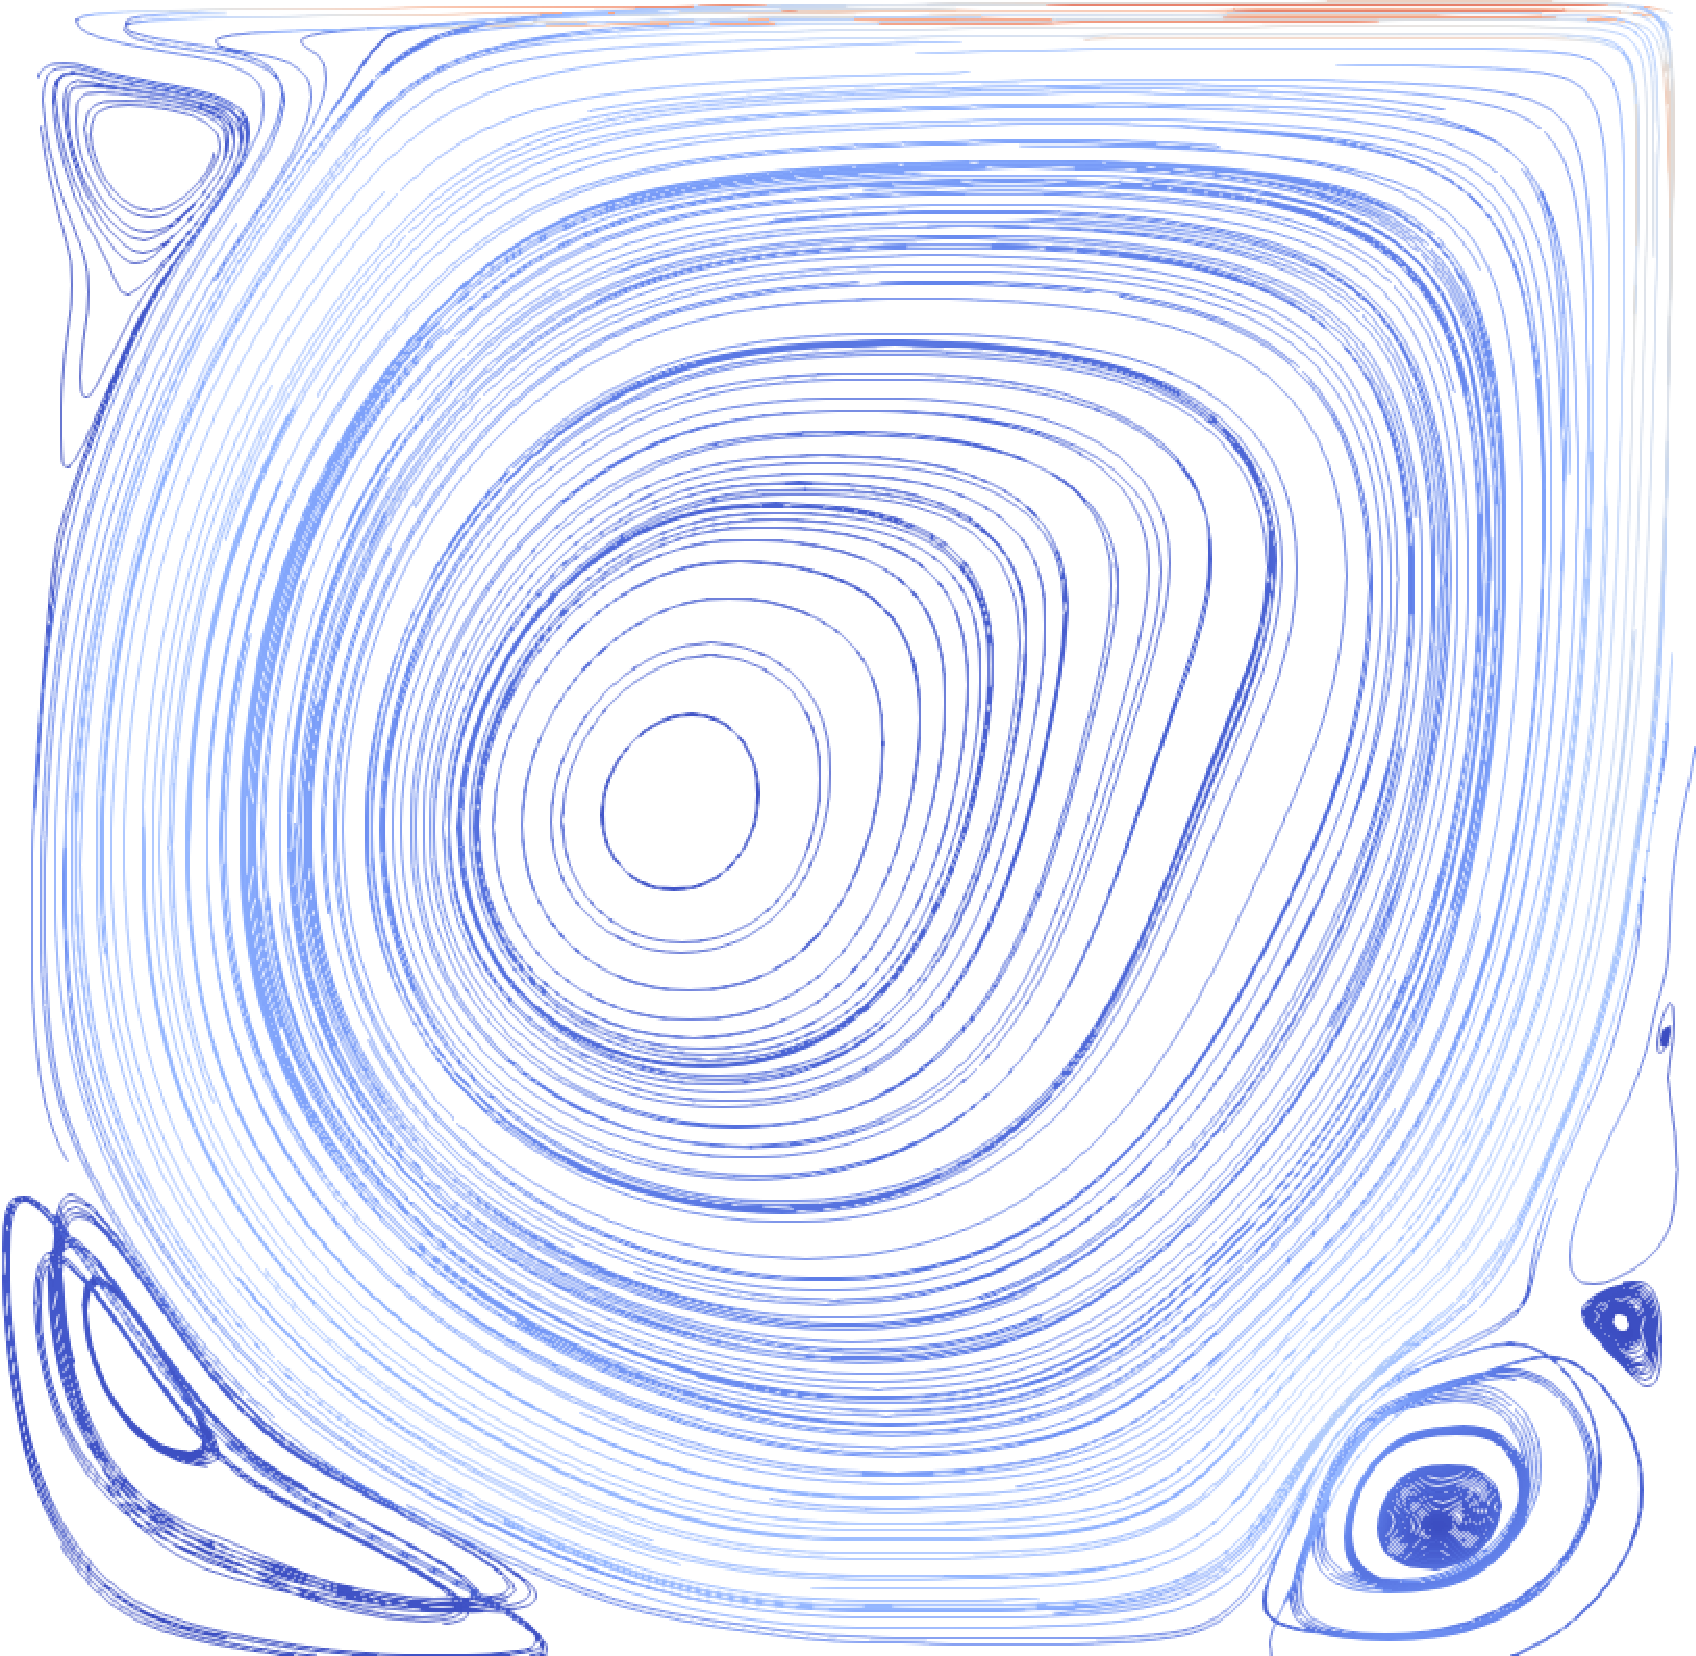
\includegraphics[width=3cm]{Results/Figure01b.pdf}
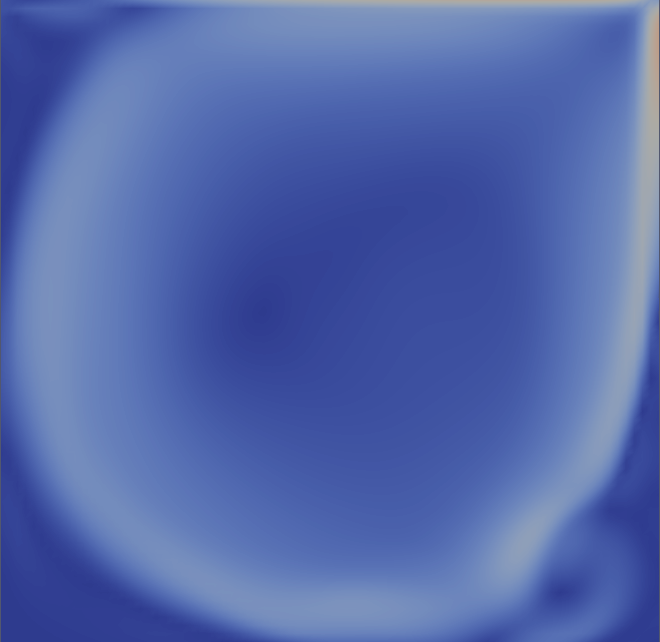
\includegraphics[width=3cm]{Results/Figure01a.pdf}
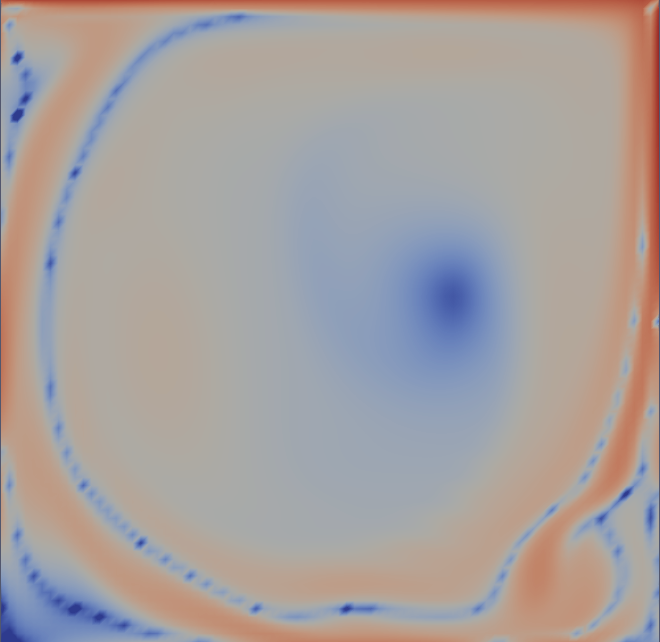
\includegraphics[width=3cm]{Results/Figure02e.pdf}
}

{
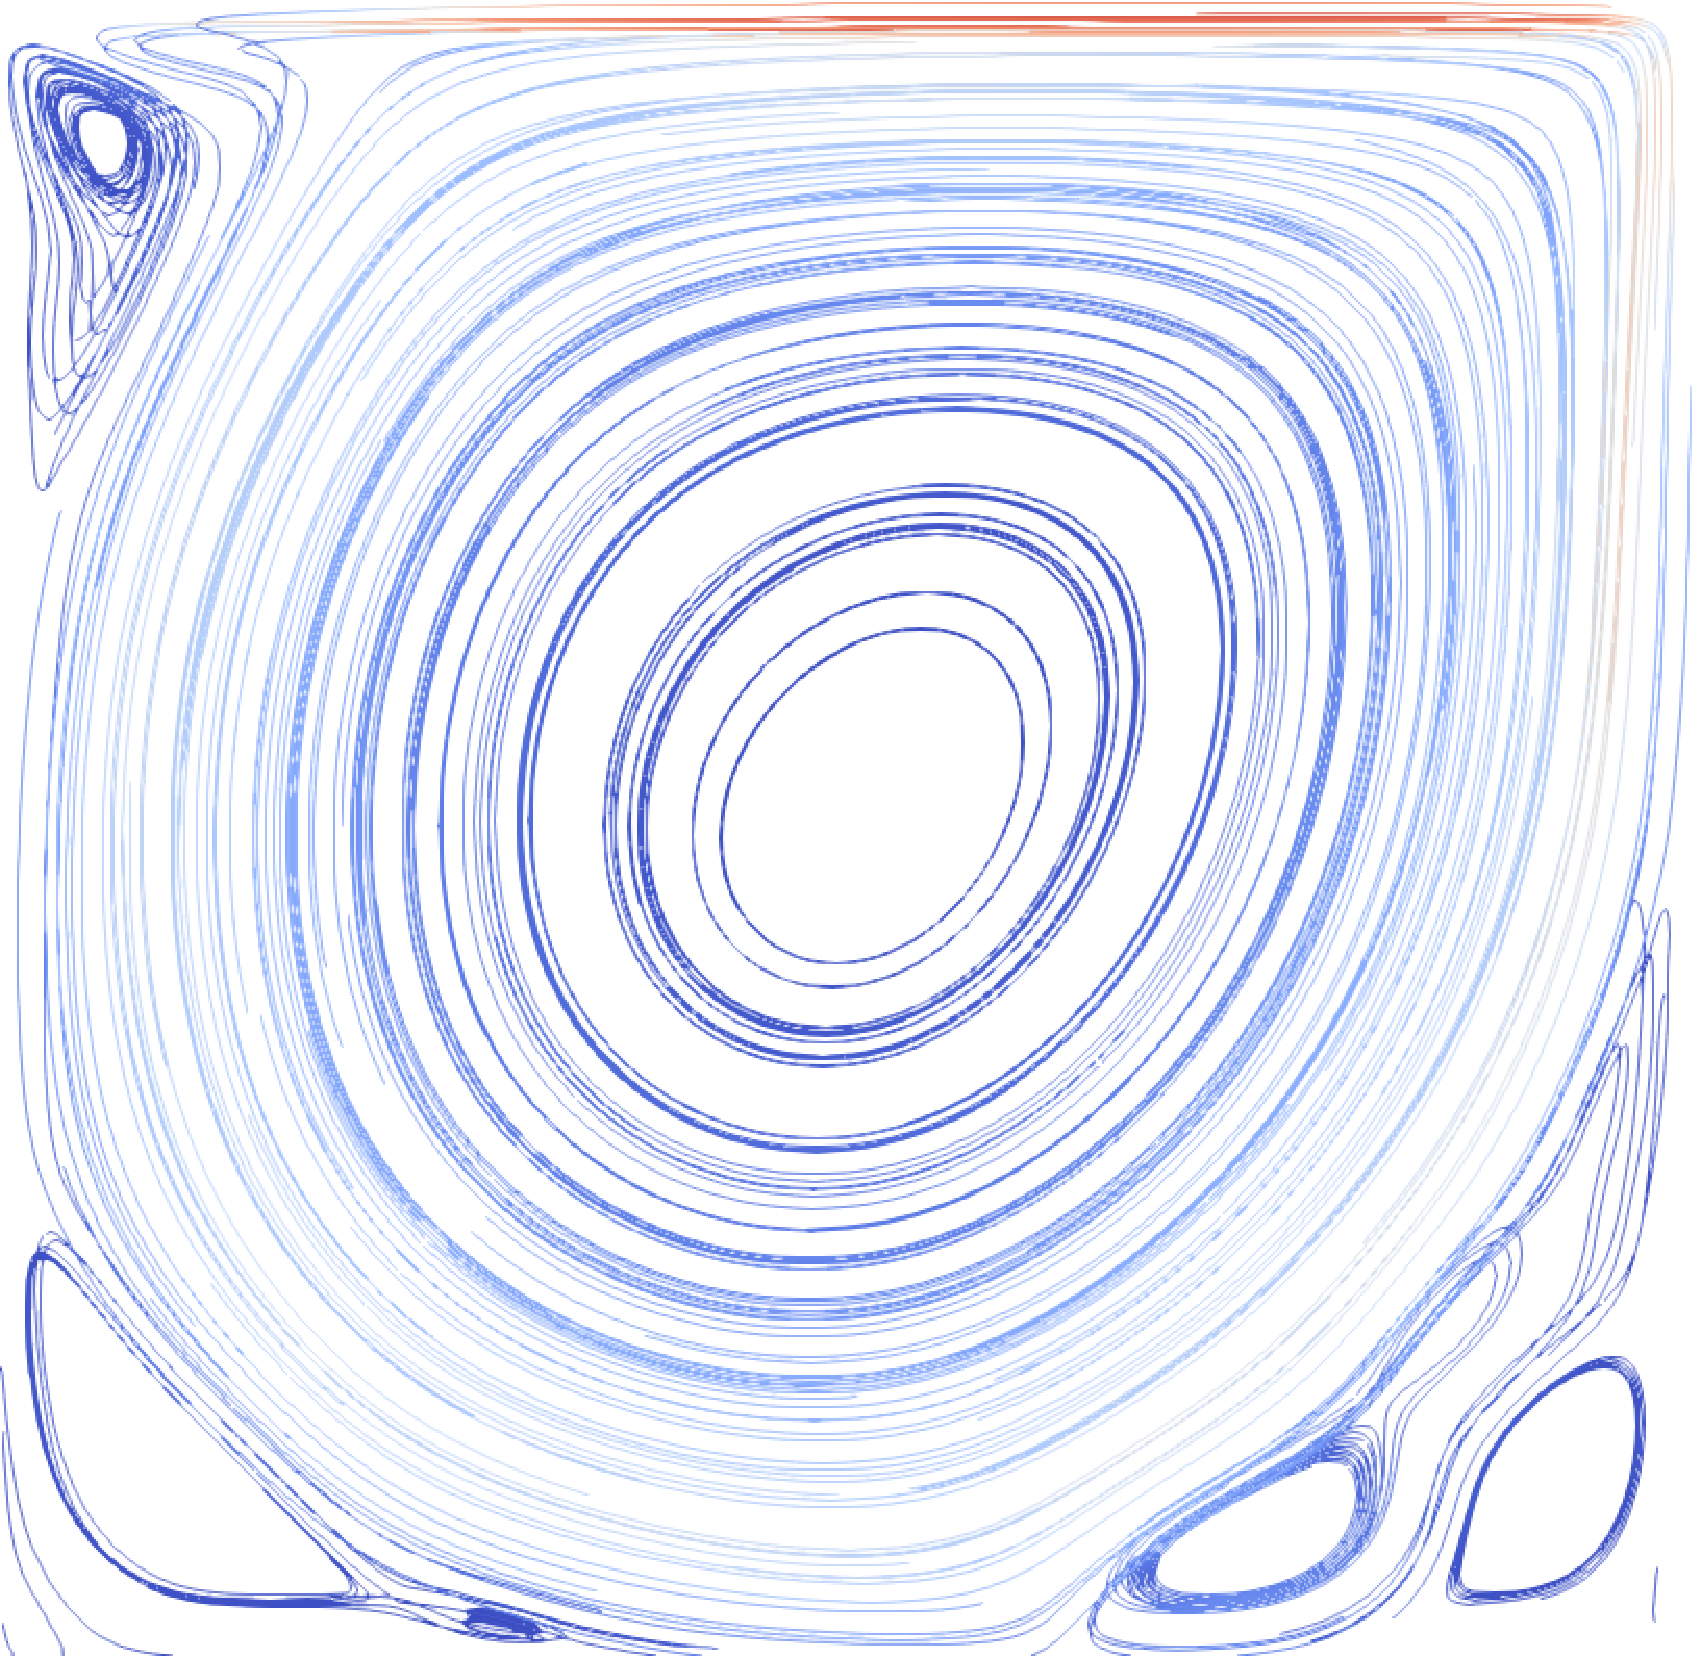
\includegraphics[width=3cm]{Results/Figure01e.pdf}
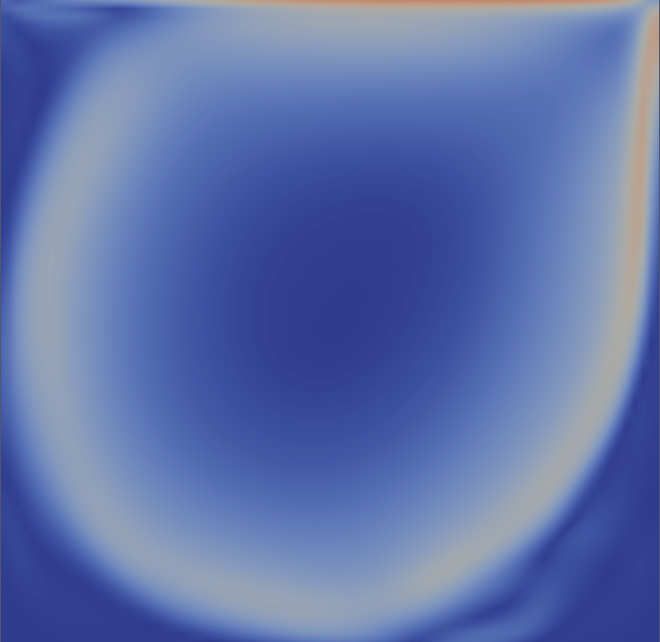
\includegraphics[width=3cm]{Results/Figure01d.pdf}
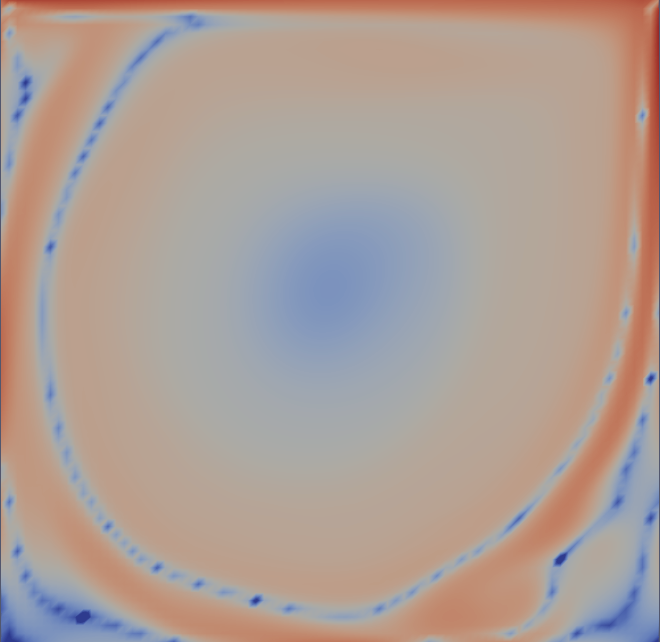
\includegraphics[width=3cm]{Results/Figure02j.pdf}
}

{
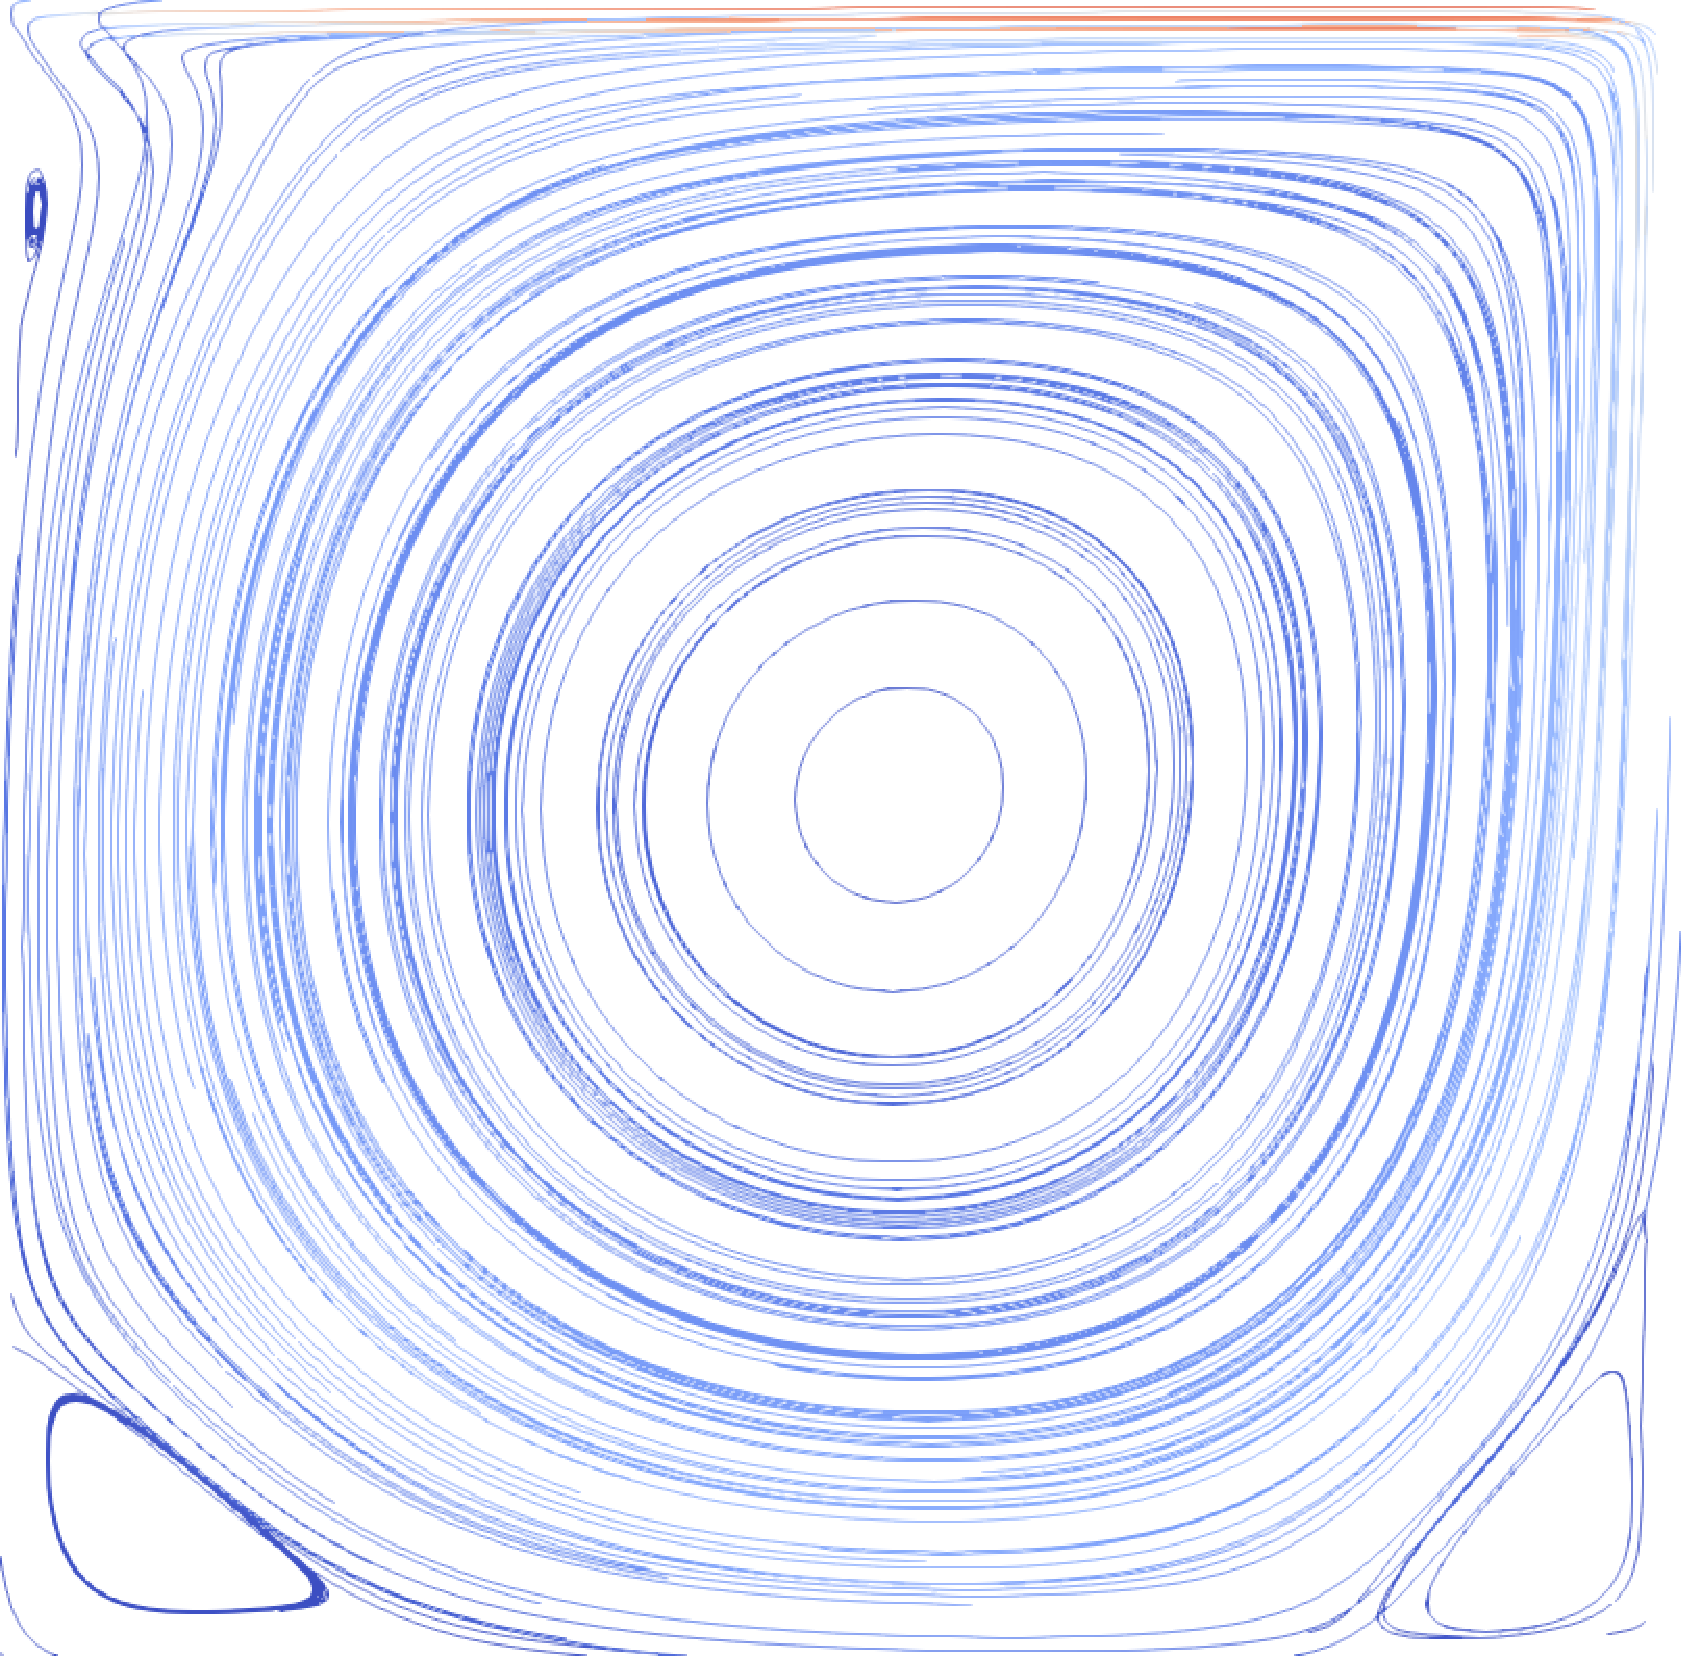
\includegraphics[width=3cm]{Results/Figure01h.pdf}
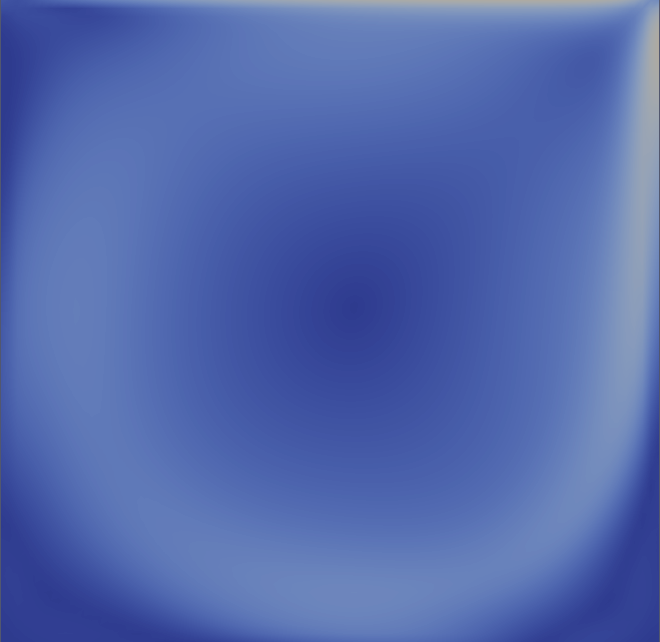
\includegraphics[width=3cm]{Results/Figure01g.pdf}
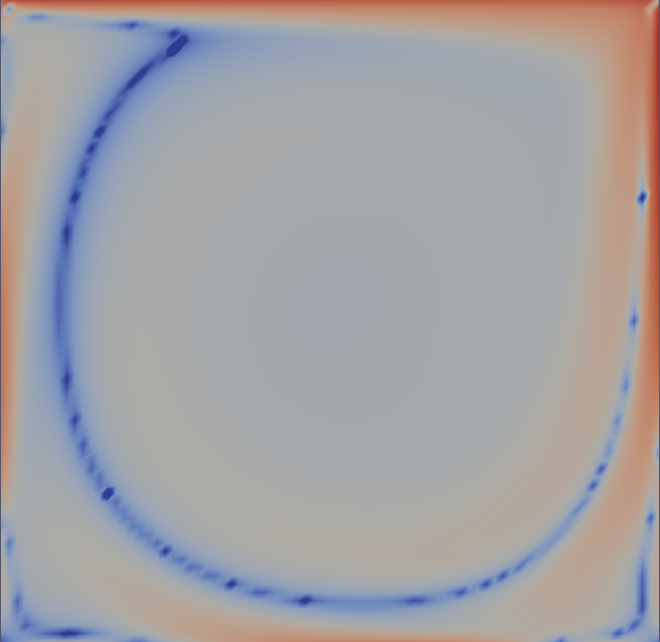
\includegraphics[width=3cm]{Results/Figure02o.pdf}
}
\caption{Simulation results at \SI{5}{s} for $ 80 \times 80 $ grid}
\label{Fig:Over}
}
{
\footnotesize
First row: DNS, second row: LES, last row: RAS. First column: flow stream lines; second column: magnitude of flow velocity $\mathbf{U}$; third column: logarithm of magnitude of vorticity $\bm{\omega}$. Blue means smaller quantities and red means larger. Best viewed in color and on digital display. (Digital version of this report can be found in \url{https://github.com/pppppass/TurbulentFlow/blob/master/Report/Report.pdf})
}
\end{figure}

From this figure, it can be easily verified that direct numerical simulation has the highest accuracy: small structures of vortexes are kept. Large eddy simulation removes some small structure, and biased the center of the largest vortex, while Reynolds-averaged simulation erases patterns of small scale almost completely.

However, to study the difference of efficiency, we have to study the dynamics of these models and related algorithms. The dynamic from \SI{1}{\second} to \SI{5}{\second} is shown in Figure \ref{Fig:Dy}.

\begin{figure}[htbp]
{
\centering
{
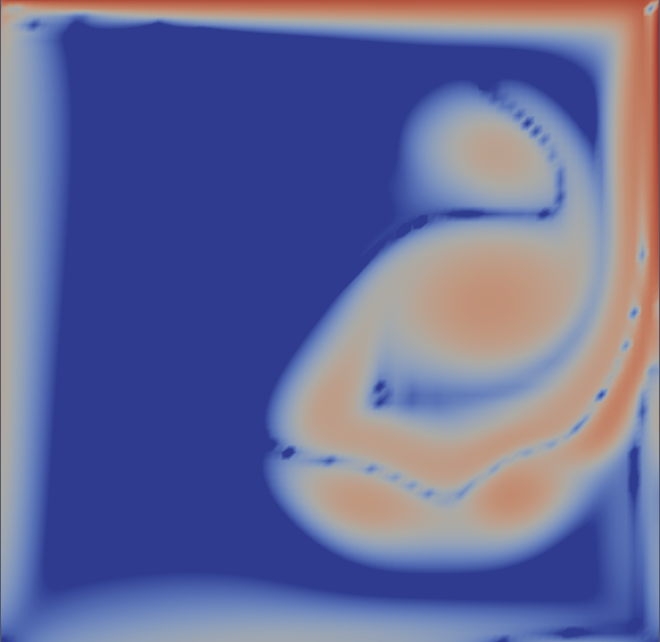
\includegraphics[width=3cm]{Results/Figure02a.pdf}
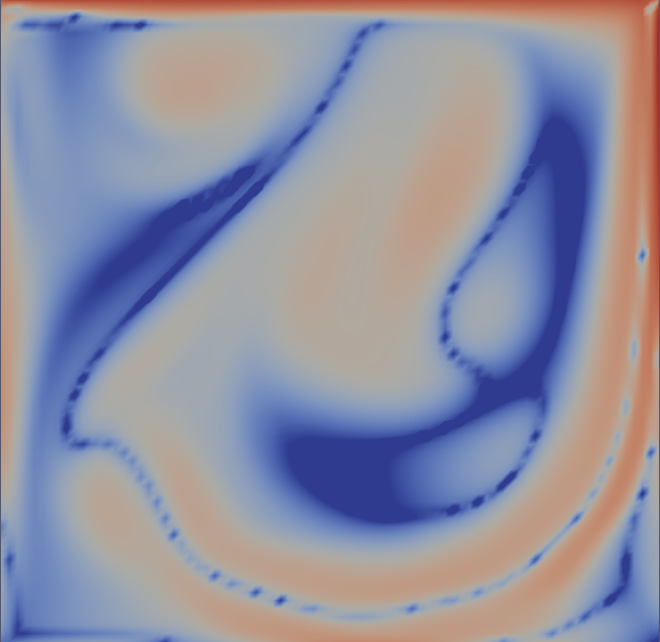
\includegraphics[width=3cm]{Results/Figure02b.pdf}
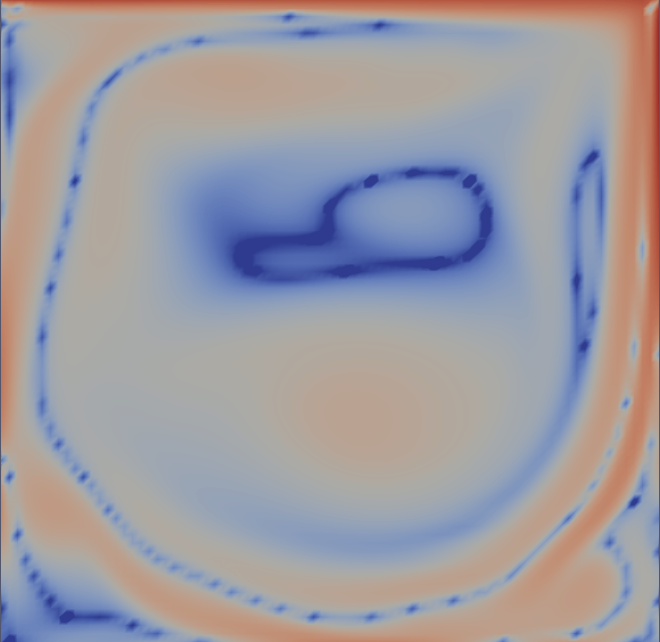
\includegraphics[width=3cm]{Results/Figure02c.pdf}
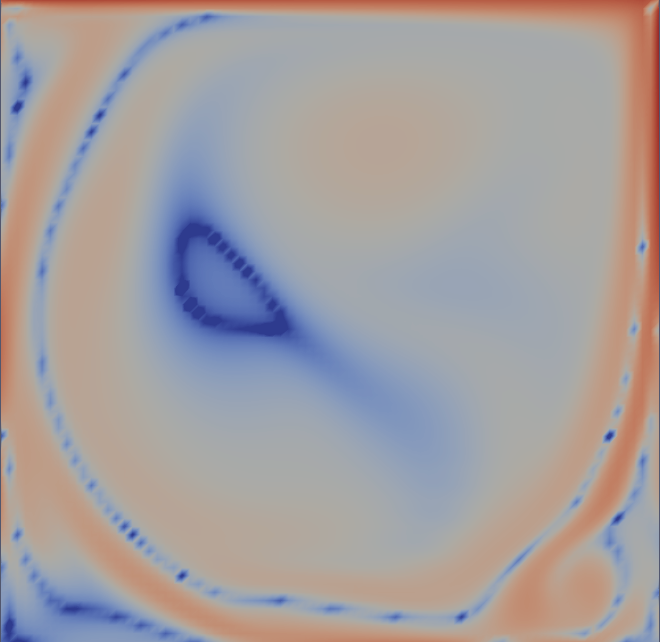
\includegraphics[width=3cm]{Results/Figure02d.pdf}
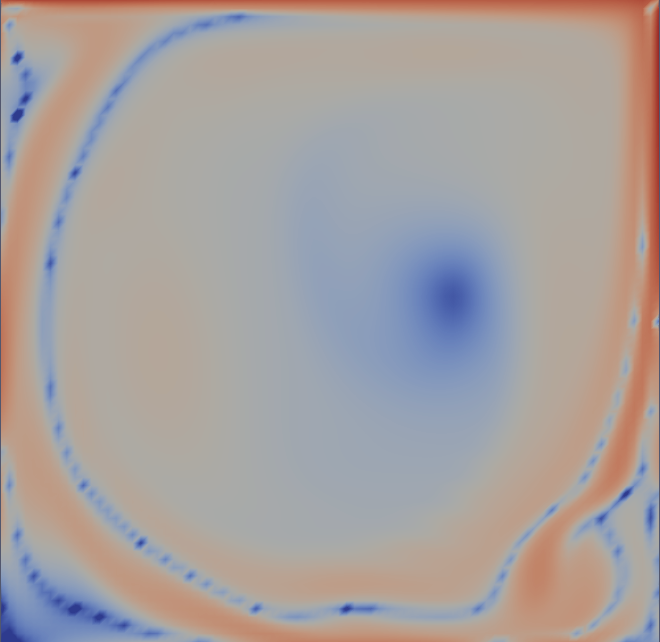
\includegraphics[width=3cm]{Results/Figure02e.pdf}
}

{
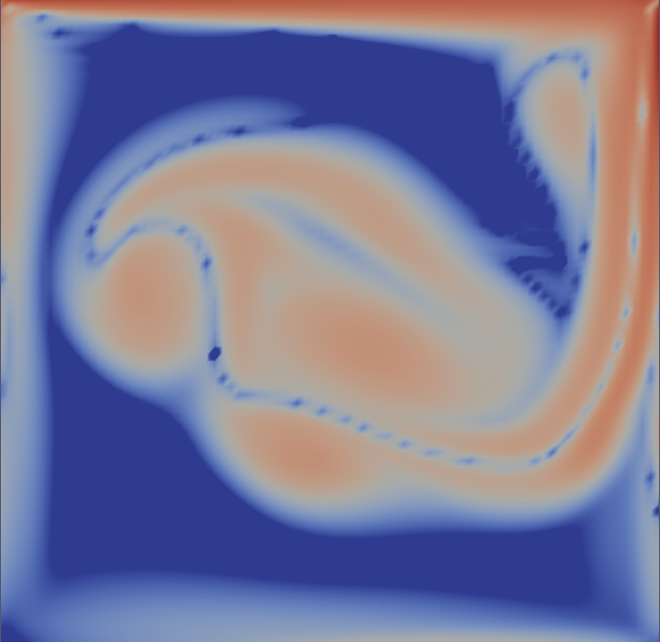
\includegraphics[width=3cm]{Results/Figure02f.pdf}
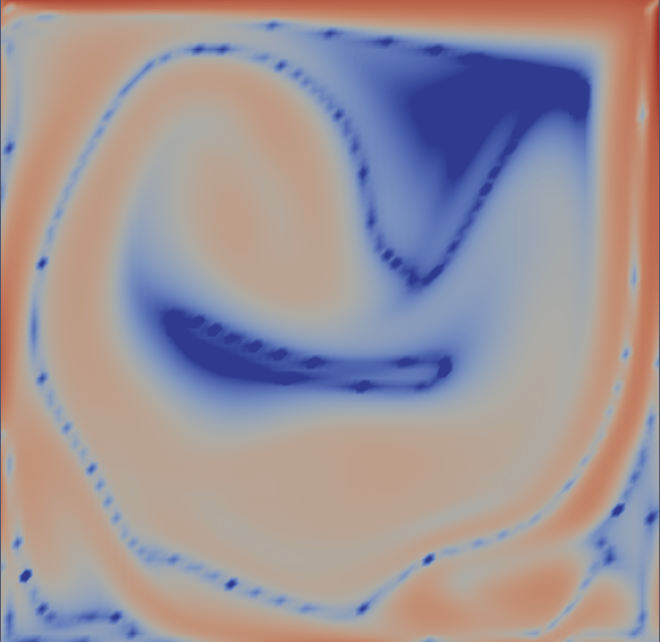
\includegraphics[width=3cm]{Results/Figure02g.pdf}
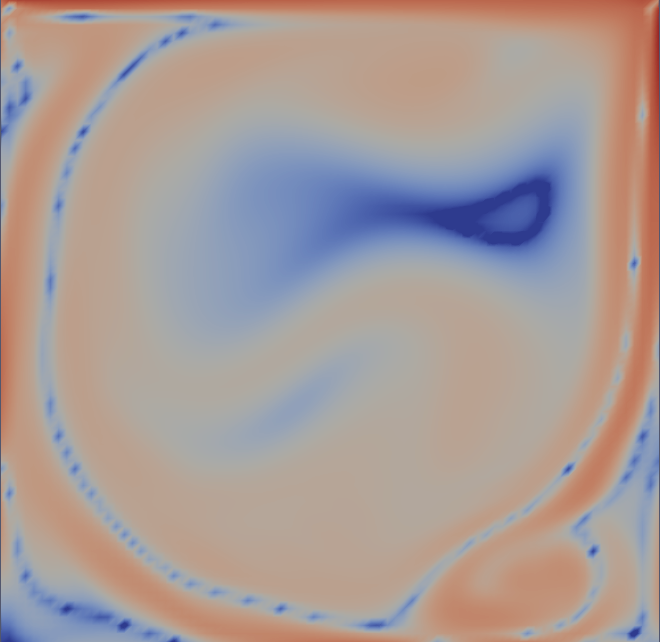
\includegraphics[width=3cm]{Results/Figure02h.pdf}
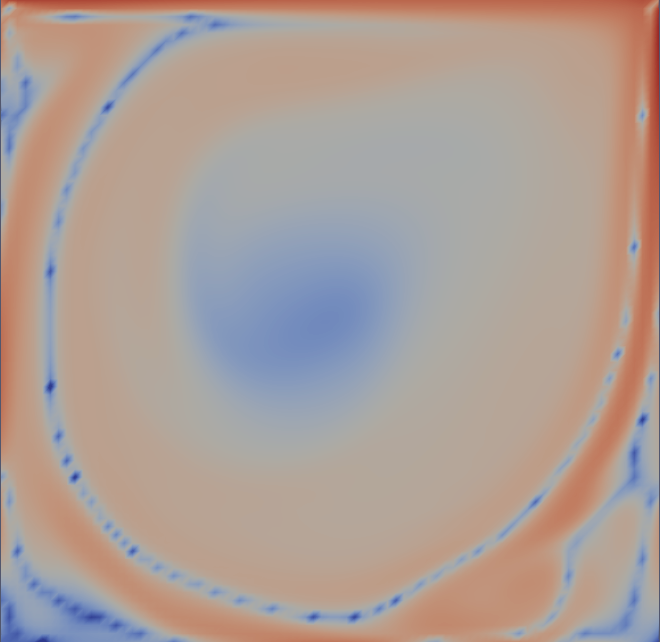
\includegraphics[width=3cm]{Results/Figure02i.pdf}
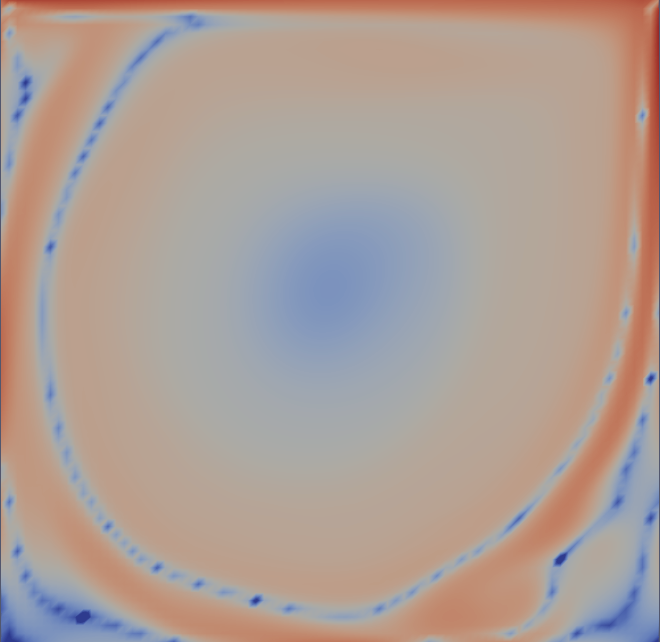
\includegraphics[width=3cm]{Results/Figure02j.pdf}
}

{
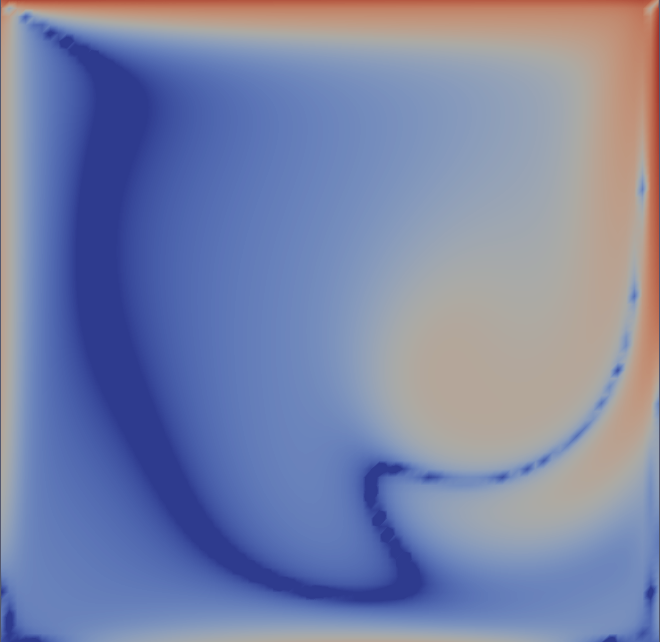
\includegraphics[width=3cm]{Results/Figure02k.pdf}
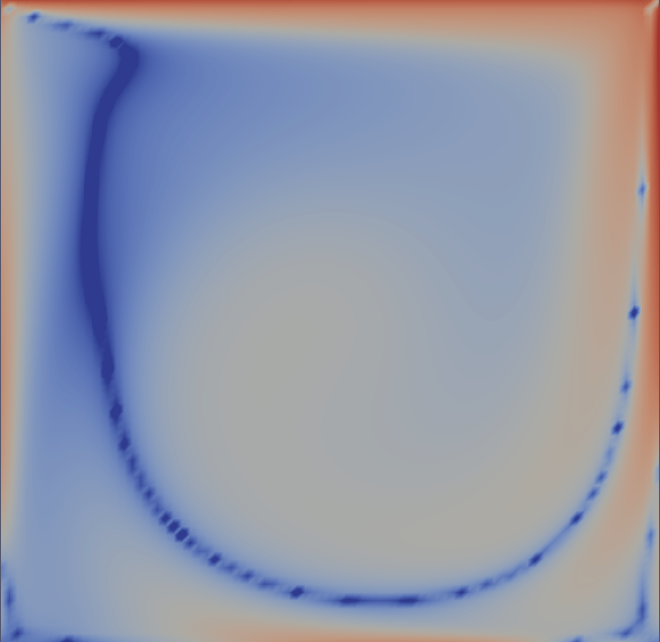
\includegraphics[width=3cm]{Results/Figure02l.pdf}
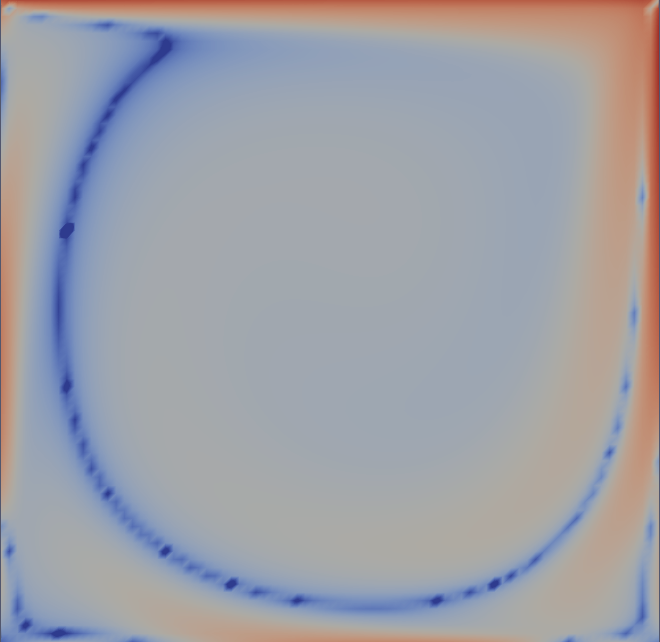
\includegraphics[width=3cm]{Results/Figure02m.pdf}
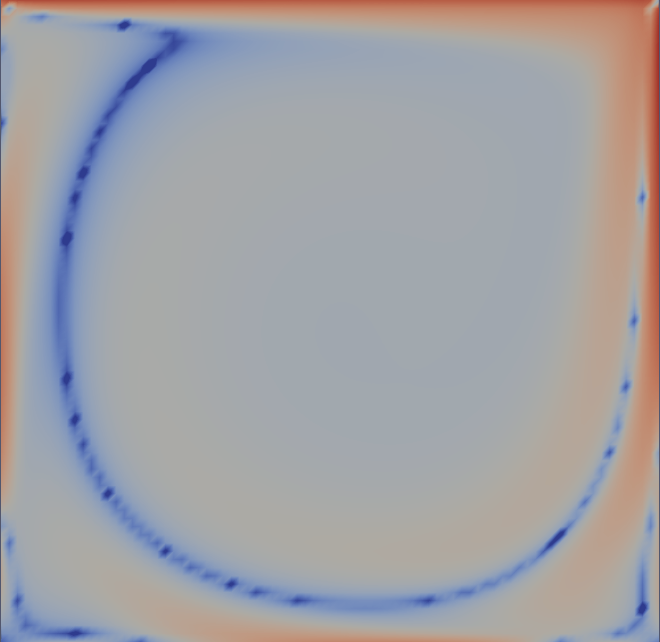
\includegraphics[width=3cm]{Results/Figure02n.pdf}
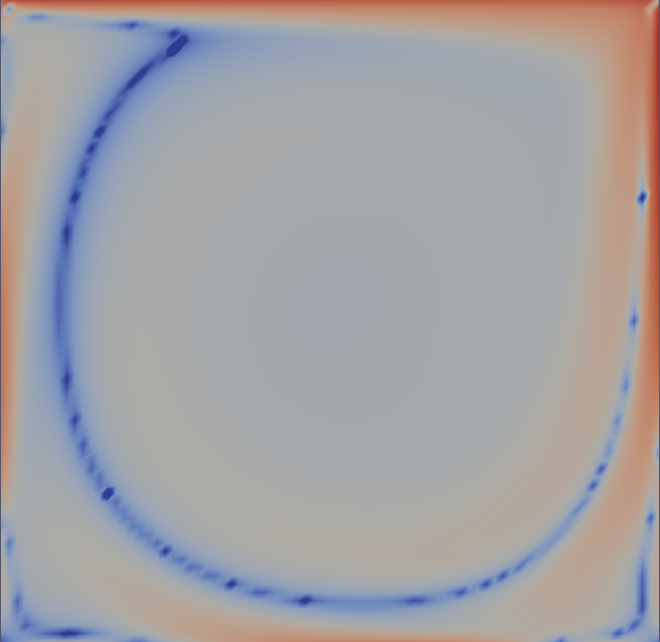
\includegraphics[width=3cm]{Results/Figure02o.pdf}
}

{
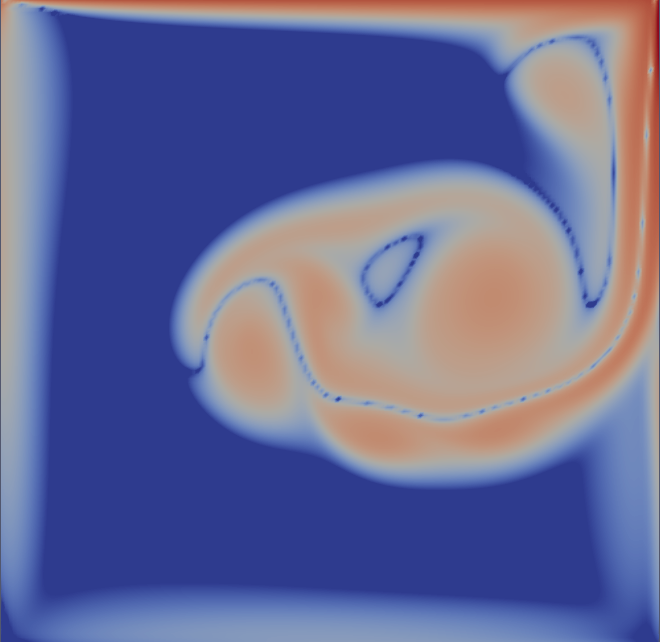
\includegraphics[width=3cm]{Results/Figure02p.pdf}
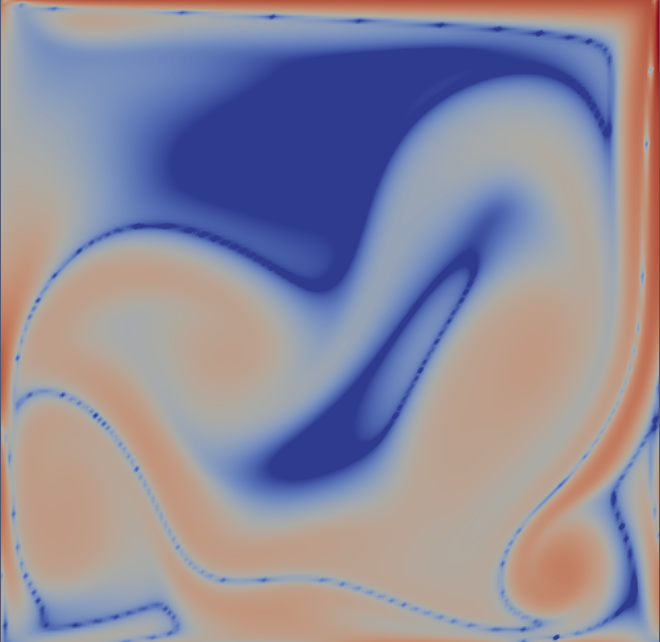
\includegraphics[width=3cm]{Results/Figure02q.pdf}
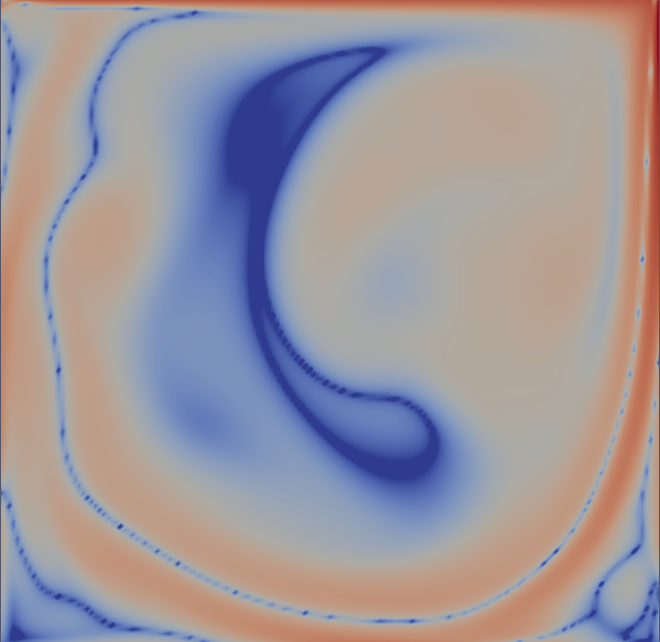
\includegraphics[width=3cm]{Results/Figure02r.pdf}
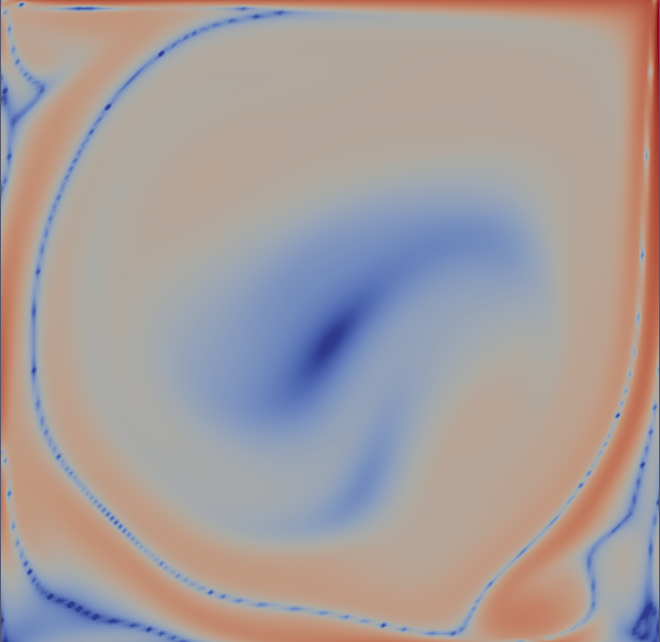
\includegraphics[width=3cm]{Results/Figure02s.pdf}
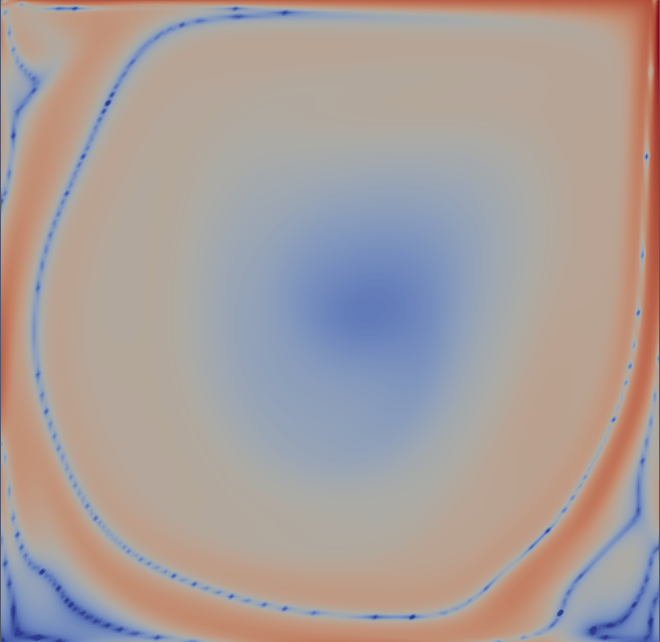
\includegraphics[width=3cm]{Results/Figure02t.pdf}
}
\caption{Simulation dynamics from \SI{1}{s} to \SI{5}{s}}
\label{Fig:Dy}
}
{
\footnotesize
These are figures of logarithm of magnitude of vorticity $\bm{\omega}$. First row: DNS for $ 80 \times 80 $ grid; second row: LES for $ 80 \times 80 $ grid; third row: RAS for $ 80 \times 80 $ grid; fourth row: DNS for $ 160 \times 160 $ grid. Columns from left to right represent 1, 2, 3, 4, \SI{5}{\second} respectively. Blue means smaller quantities and red means larger. Best viewed in color and on digital display.
}
\end{figure}

From this figure, it can be directly observed that the direct numerical simulation on coarse grids does not converge into the stationary solution rapidly. On the contrary, the solution of large eddy simulation and Reynolds-averaged simulation converges faster because of the introduction of space or time averages. It is clear that Reynolds-averaged simulation gets stable in two seconds, and this proves that this simulation model can capture statistical steadiness. Another important comparison is between the first, second and fourth row: the result of direct numerical simulation on the fine grid is more similar to the result large eddy simulation on the coarse grid, especially at \SI{1}{\second} and \SI{5}{\second}. This tells the success of multi-scale modeling of large eddy simulation: the structures of small scales are directly modeled rather than computed, and therefore it is possible to simulation on a coarse grid using large eddy simulation as if direct numerical simulation is performed on a fine grid. This highly increases efficiency and cuts down computations.

We summarize the running time for different simulation models and grid sizes. This is shown in Table \ref{Tbl:Run}.

\begin{table}[htbp]
\centering
\caption{Comparison on running time (\Si{\second})}
\label{Tbl:Run}
\begin{tabular}{|c|c|c|c|}
\hline
Grid size & DNS & LES & RAS \\
\hline
$ 20 \times 20 $ & 4.62 & 5.19 & 6.16 \\
\hline
$ 40 \times 40 $ & 21.84 & 25.56 & 28.20 \\
\hline
$ 80 \times 80 $ & 161.82 & 174.46 & 198.67 \\
\hline
$ 160 \times 160 $ & 1380.04 & 1564.41 & 1890.42 \\
\hline
\end{tabular}
\end{table}

Because the number of equations gets larger for large eddy simulation and Reynolds-averaged simulation, the running time also becomes longer. However, one should not forget about the grid size: from previous arguments, large eddy simulation behaves well on coarse grid, and significantly cuts down the running time. For Reynolds-averaged simulation, the system gets stable in a fast sense, and the simulated time can also be noticeably decreased. If we want to find the statistically stationary solution , Reynolds-averaged simulation can be even faster.

We the examine the example of flows over a cylinder. The cylinder of radius \SI{0.5}{\meter} is placed into a 2-dimensional rectangular flow pipe of width \SI{2}{\meter}. The center of cylinder section is \SI{2}{\meter} to the inlet and \SI{18}{\meter} to the outlet. The inlet provides flow of velocity $ U_0 = \SI{1}{\meter\per\second} $. To break the symmetry, we add $ U'_0 = \SI{0.1}{\meter\per\second} $ vertically (the $y$ axis). The kinetic viscosity is $ 5 \times 10^{-4} \Si{\squared\meter\per\second} $. As a result, the Reynolds number is about 3000 (considering the half upper region and ignore $U'_0$).

The simulation result is shown in Figure \ref{Fig:Cyl}. K\'arm\'an vortex street can be observed.

\begin{figure}[htbp]
{
\centering
{
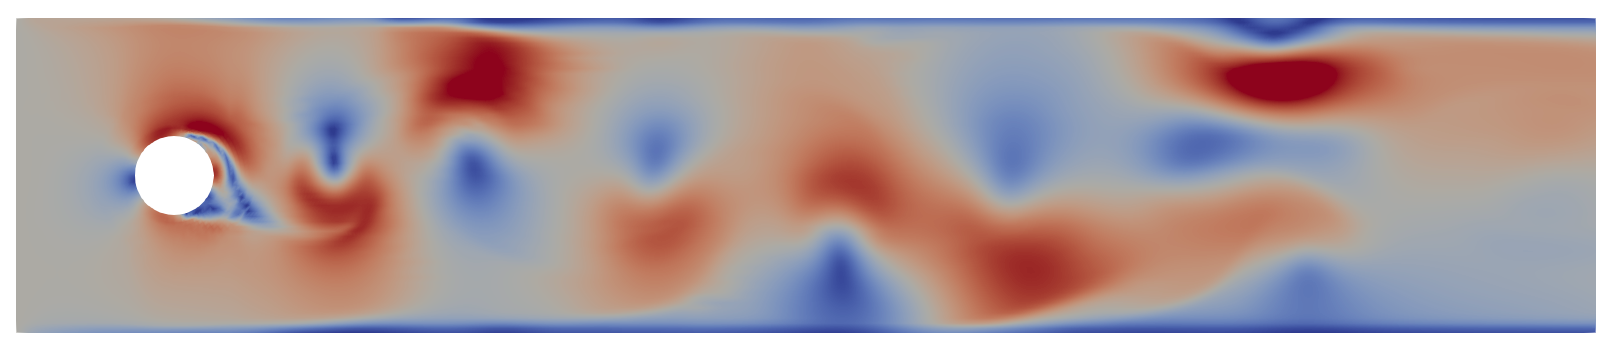
\includegraphics[width=15cm]{Results/Figure03a.pdf}
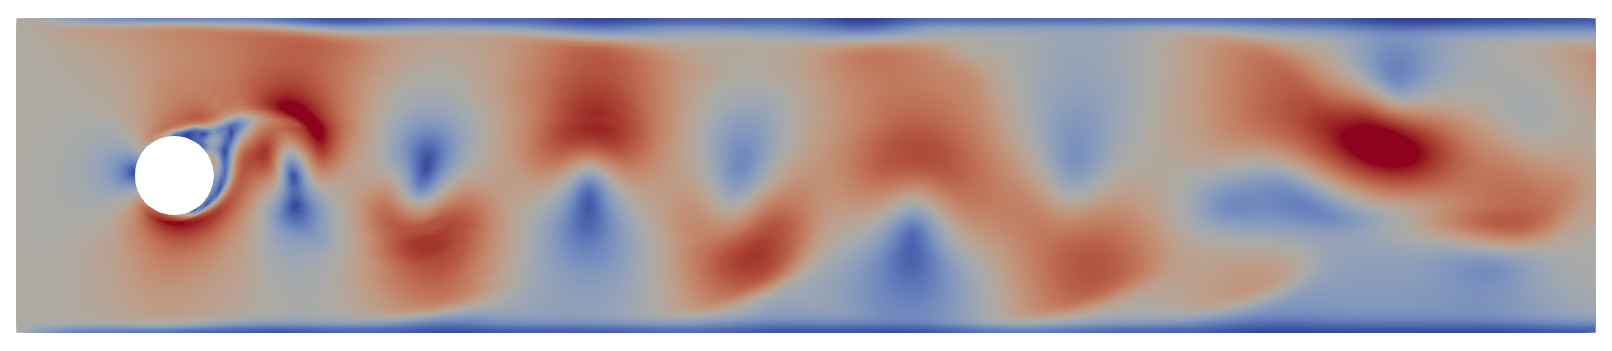
\includegraphics[width=15cm]{Results/Figure03b.pdf}
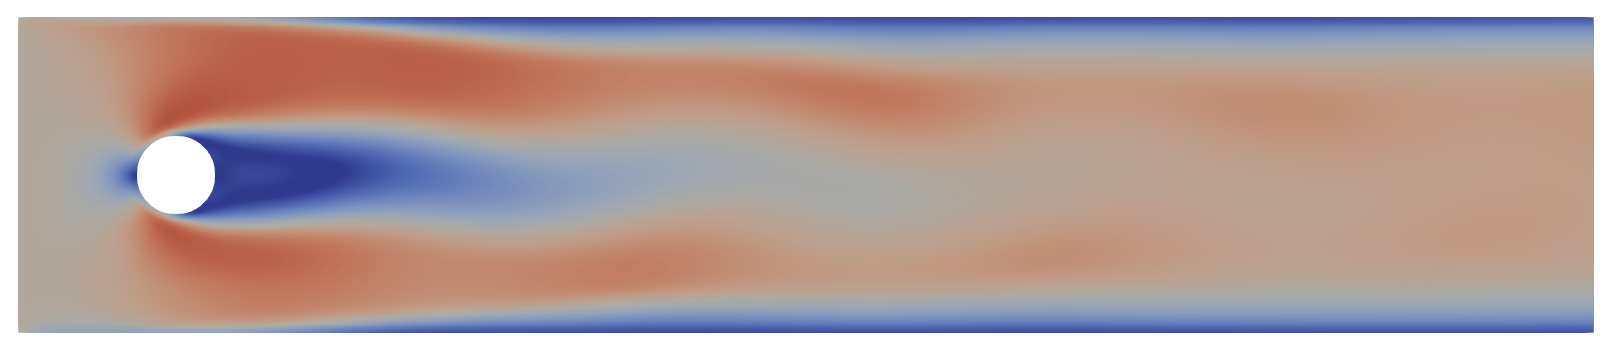
\includegraphics[width=15cm]{Results/Figure03c.pdf}
}
\caption{Simulations result of flows over a cylinder at $\SI{20}{\second}$}
\label{Fig:Cyl}
}
{
\footnotesize
These are figures of magnitude of flow velocity $\mathbf{U}$. First row: DNS; second row: LES; last row: RAS. Blue means smaller quantities and red means larger. Best viewed in color and on digital display.
}
\end{figure}

In this figure, the distinction among these three models are again magnified. The comparison between the first two rows shows that the vortex street of large eddy simulation is more regular and continuous, while that of direct numerical simulation introduces some artifacts here. To be exact, the vortex street in direct numerical simulation gets broken up and the size of vortexes varies a lot, which is not expected. This is because the size of grids does not reach three fourth power of the Reynolds number, as mentioned above, and therefore direct numerical simulation cannot capture such details. For large eddy simulation, part of the vortexes are modeled and therefore accuracy and regularity can be preserved. Note that Reynolds-averaged simulation fails here, because the profile itself does not have statistical steadiness: it has periodical movement after all.

These results are carried out on a computer with Intel Core i7-6500U (4 threads) and $\SI{7886}{\mebi\byte}$ RAM. The operating system is Arch Linux 4.16.13 64-bit. We deploy OpenFOAM 5.0 \parencite{weller_tensorial_1998} for numerical simulation. Detailed settings including initial values, boundary conditions and numerical schemes are provided in \url{https://github.com/pppppass/TurbulentFlow/tree/master/Experiments}.

\subsection{Further discussion and novel ideas}

We present some further discussion about the three models and present a novel idea for turbulent flow modeling in this sub-section.

Generally speaking, the Reynolds-averaged simulation is ``one point correlation'' model, which pays attention on the probability distribution of velocity (and pressure) on one point. In the work related to Kolmogorov \parencite{kolmogorov_equations_1941} \parencite{sreenivasan_universality_1995} \parencite{pope_turbulent_2001}, statistical behavior of two point is analyzed to get the energy spectrum. However, such ``two points correlation'' model is under development. The computational difficulty lies here because the problem size get squared, and also it is not clear about how we can utilize the correlation of velocity of a pair of points.

In another sense, the large eddy simulation model emulates the correlation among points of a local area: it makes use of a filter and try to stablize the quantities. However, the filter is directly given: it force use to filter out fine details, or say some special kind of correlation is retained. This leads to the loss of high frequency signals.

Another problem should also be considered. For Reynolds-averaged simulation, we have only the expectation, say Reynolds-averaged velocity $\pbr{U_i}$ and the covariance matrix, say Reynolds stress $ \pbr{ U_i U_j } $ for the three-dimensional random variable $\mathbf{U}$. Therefore, it is rather impossible to capture the probability distribution, without statistical hypothesis of Gaussian distribution. However, it can be a problem, if we want to find the ``statistical stable'' solution and then generated random configuration of $\mathbf{U}$ from it. In other words, only the expectation and covariance can be solved, and real turbulent flows cannot be simulated from Reynolds-averaged simulation model. The failure of flows over a cylinder also exemplifies this issue.

All problems boil down to capture a complicated probability distribution. In the communities of statistics and machine learning, there are a lot of methods to emulate and sample from a probability distribution. Recent development of machine learning and deep learning shows the potential of such distribution probability of data-driven methods. Additionally, according to the first hypothesis of Kolmogorov \parencite{kolmogorov_equations_1941}, the turbulent flows of small scales are independent to each other, and therefore some locality is inherited then.

Borrowing the ideas of data-driven methods, which worths a trial is to use a generative model to capture the probability distribution of turbulent flows. Such generative model can be a deep belief network \parencite{hinton_fast_2006} \parencite{lee_convolutional_2009} or a deep Boltzmann machine \parencite{salakhutdinov_restricted_2007} \parencite{nair_rectified_2010} \parencite{salakhutdinov_efficient_2010}. Recent development in deep learning also provides us generative models like variational autoencoders \parencite{kingma_auto-encoding_2013} \parencite{doersch_tutorial_2016} and generative adversarial networks \parencite{goodfellow_nips_2016} \parencite{arjovsky_wasserstein_2017}. Physics law should also be considered as constrains. This means that we need to carefully design the architecture of generative model. We may use sampling techniques like Monte Carlo Markov Chain to emulate turbulent flows.

In conclusion, we may combine statistical models or data-driven models to capture the probability distribution of turbulent flows, including both many-point correlation and detailed density distribution of velocity. The key idea is to use a generative model to capture the chaos and relative probability distributions, with physics laws coupled. Such model is expected to capture the chaotic behavior of turbulent flows, and thus provides us a new aspect of turbulent flow simulation. This is a recently developed idea for novelty, and further research may be carried on.

\section{Conclusion} \label{Sec:Con}

This report presents an introduction to turbulent simulation, including the mathematical formulation and three different models: direct numerical simulation, large eddy simulation and Reynolds-averaged simulation. Comparison among these three models are also showed in this report. We also present detailed analysis and numerical experiments on various cases with these three models, and show the distinctions among these models.

Turbulent flows are of high importance in computational mathematics and engineering. It is also an interesting question whether it is possible to combine classical models with recent popular learning-based algorithms. One of the key challenge for learning-based algorithms is to ``learn'' the model directly. After all, in some sense, the problem of turbulent flows is main a problem of models.

\section{Acknowledgement} \label{Sec:Ack}

Ten days ago, we had no acquaintance with anything in the field of computational fluid dynamics and turbulent flow simulation at all. Although we finished the literature survey and comparative analysis and experiments on our own, we express our thanks to Zexing Li, whose talk initiated us to begin such an adventure.

\section{Reference}

\printbibliography

\end{document}
